\documentclass[12pt,a4paper]{report}

\usepackage[slovak]{babel}
\usepackage[utf8]{inputenc}
\usepackage[T1]{fontenc} 
%\usepackage[IL2]{fontenc} 
\usepackage{a4wide}
\usepackage{tabularx}
\usepackage{amsfonts}
\usepackage{amssymb}
\usepackage{amsmath}
\usepackage{amsthm}
\usepackage{epsfig}
\usepackage{color}
\usepackage{mathrsfs}
\usepackage{verbatim}
\usepackage{float}
\usepackage{longtable}
\usepackage{multicol}
\usepackage{graphicx}
\usepackage{pdfpages}
\usepackage{lastpage}
\usepackage{standalone}
\usepackage{url}
\usepackage{courier}
\usepackage[small,bf]{caption}
\usepackage{dirtree}
\usepackage{fixltx2e}
\usepackage{enumerate}
\usepackage{mathtools}
%\usepackage{tikz}
%\usetikzlibrary{arrows,%
%                petri,%
%                topaths}%
%\usepackage{tkz-berge}
%\usepackage{../pkg/tikz-uml}

% zadefinovanie prikazu \todo
\newcommand\todo[1]{\textcolor{red}{TODO: #1}}

% nastavenie hlaviciek a paticiek
\usepackage{fancyhdr}
\pagestyle{fancy}
\lhead{}
\rhead{\nouppercase{\textsc{\leftmark}}}
%\makeatletter
\renewcommand{\chaptermark}[1]{\markboth{\thechapter.\ #1}{}}
%\makeatother

%\makeatletter
%\let\ps@plain\ps@fancy
%\makeatother
%\usepackage[pdfpagelabels]{hyperref}

% nastavenie velkosti okrajov, riadkovania
\setlength{\textheight}{24cm}
\setlength{\textwidth}{15.5cm}
\addtolength{\voffset}{-1.2cm}
\addtolength{\hoffset}{0cm}
\setlength{\parindent}{0.5cm}
\setlength{\parskip}{0in}
\setlength{\headheight}{16pt}
\linespread{1.3}

% nastavenie cross referencii
\usepackage{hyperref}                                     
\hypersetup{
    unicode=true,
    bookmarksnumbered,
    pdfstartview={FitH},
    linkcolor=black,
    citecolor=black,
    colorlinks=true,
    urlcolor=black
}

% nastavenie includovania obrazkov cez \includesvg
\graphicspath{{../img/}}
\newcommand{\includesvg}[1]{
    \immediate\write18{inkscape -z -D –file=../img/#1.svg
    –export-pdf=img/#1.pdf –export-latex}
    \input{../img/#1.pdf_tex}
}

% nastavenie 'code' environmentu
\usepackage{listings}
\renewcommand\lstlistlistingname{Zoznam listingov}
\definecolor{gray}{rgb}{0.5,0.5,0.5}
\definecolor{dgray}{rgb}{0.35,0.35,0.35}
\lstnewenvironment{code}[1][]%
{
%    {\minipage{\linewidth}
        \lstset{        
            commentstyle=\color{dgray}\textit,
            escapeinside={<*}{*>},
            showstringspaces=false,
            %aboveskip=20pt, % HACK
            %xleftmargin=10pt,
            %xrightmargin=10pt,
            frame=single,
            basicstyle=\small\ttfamily,
            numberstyle=\small\color{gray},
            numbers=left,
            captionpos=b,
            language=C++,
            #1
        }
%    }
%    {\endminipage}
}{}

\lstnewenvironment{pseudocode}[1][]%
{
%    {\minipage{\linewidth}
        \lstset{        
            morecomment=[l]{\#},
            commentstyle=\color{dgray}\textit,
            escapeinside={<*}{*>},
            showstringspaces=false,
            %aboveskip=20pt, % HACK
            %xleftmargin=10pt,
            %xrightmargin=10pt,
            frame=single,
            basicstyle=\small\ttfamily,
            numberstyle=\small\color{gray},
            numbers=left,
            captionpos=b,
            #1
        }
%    }
%    {\endminipage}
}{}

% nastavenie definicii atd 
% TODO mozno to dajak inak dat
\theoremstyle{plain}
\newtheorem{defn}{Definícia}[chapter] 

\theoremstyle{plain}
\newtheorem{ozn}{Označenie}[chapter] 

\theoremstyle{plain}
\newtheorem{theorem}{Veta}[chapter]

\theoremstyle{plain}
\newtheorem{lemma}[theorem]{Lemma}

\theoremstyle{definition}
\newtheorem{example}{Príklad}[chapter]

\theoremstyle{definition}
\newtheorem{pozn}{Poznámka}[chapter]

\begin{document}

    \pagenumbering{roman}
    
    \thispagestyle{empty}

\begin{center}
    \large{
        \textsc{
            Univerzita Komenského v Bratislave \\
            Fakulta matematiky, fyziky a informatiky
        }
    }
\end{center}

\vspace{2cm}

\begin{figure}[!h]
    \centering
    
\includegraphics[width=3.5cm]{komlogo-new}
\end{figure}

\vspace{1cm}

\begin{center}
    \LARGE{
        \textbf{
            \textsc{
                Dátové štruktúry pre uchovávanie \\
                sekvenovacích dát \\
            }
        }
    }
    \vspace{1cm}
    \large{
        \textsc{
            Diplomová práca
        }
    }
\end{center}

\vfill

\begin{multicols}{2}
    \begin{flushleft}
        \textbf{\the\year}
    \end{flushleft}
    \begin{flushright}
        \textbf{Bc. Jakub JURSA}
    \end{flushright}
\end{multicols}
    \newpage
\thispagestyle{empty}

\begin{center}
    \large{
        \textsc{
            Univerzita Komenského v Bratislave \\
            Fakulta matematiky, fyziky a informatiky
        }
    }
\end{center}

\vspace{5cm}

\begin{center}
    \LARGE{
        \textbf{
            \textsc{
                Dátové štruktúry pre uchovávanie \\
                sekvenovacích dát \\
            }
        }
    }
    \vspace{1cm}
    \large{
        \textsc{
            Diplomová práca
        }
    }
\end{center}

\vfill

\begin{center}
    \begin{tabular}{ll}
        Študijný program:               &   Informatika \\
        Študijný odbor:                 &   2508 Informatika \\
        Školiace pracovisko:            &   Katedra informatiky \\
        Školiteľ:                       &   Mgr. Tomáš Vinář, PhD. \\
        Konzultant:                     &   Mgr. Vladimír Boža \\
    \end{tabular}
\end{center}

\vfill

\begin{multicols}{2}
    \begin{flushleft}
        \textbf{Bratislava \the\year}
    \end{flushleft}
    \begin{flushright}
        \textbf{Bc. Jakub JURSA}
    \end{flushright}
\end{multicols}
    \newpage

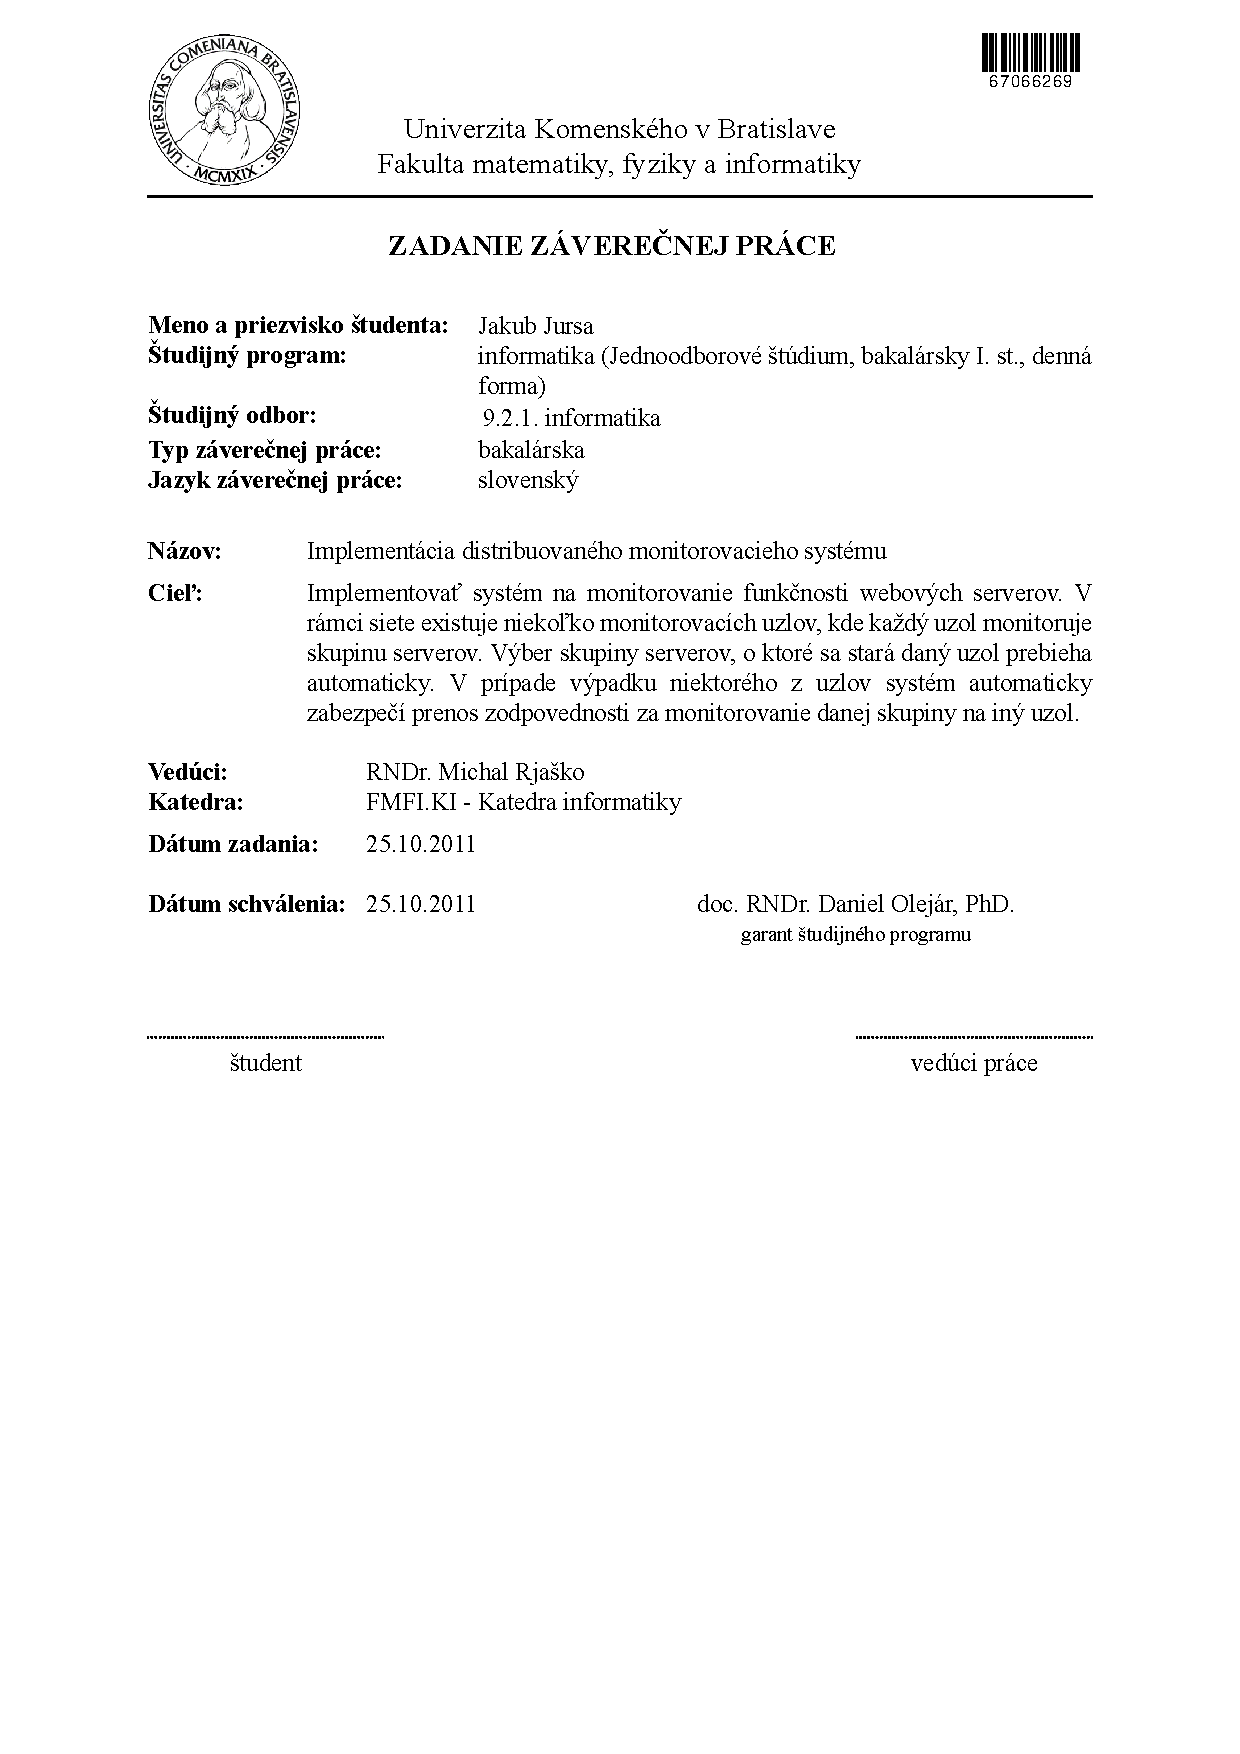
\includepdf[offset=0 -80]{zadanie.pdf}
    \newpage

\section*{Poďakovanie}
Ďakujem konzultantovi mojej diplomovej práce, Mgr. Vladimírovi Božovi za jeho rady, trpezlivosť a pripomienky pri písaní tejto práce.
    \newpage

\section*{Abstrakt}

\begin{tabular}{ll}
    \textbf{Autor:}                       & Jakub Jursa \\
    \textbf{Názov diplomovej práce:}      & Dátové štruktúry pre uchovávanie
    sekvenovacích dát \\
    \textbf{Škola:}                       & Univerzita Komenského v
                                            Bratislave \\
    \textbf{Fakulta:}                     & Fakulta matematiky, fyziky a
                                            informatiky \\
    \textbf{Katedra:}                     & Katedra informatiky \\
    \textbf{Vedúci diplomovej práce:}     & Mgr. Tomáš Vinař, PhD. \\
    \textbf{Konzultant diplomovej práce:} & Mgr. Vladimír Boža \\
    \textbf{Rozsah práce:}                & \pageref{LastPage} strán \\
    \\
    Bratislava, máj \the\year             & {} \\
    \\
    \multicolumn{2}{p{15.3cm}}{
        \emph{Sem pribudne abstrakt \ldots}
    }\\
    \\        
    \textbf{Kľúčové slová:}             &  \emph{kľúčové slová \ldots}
\end{tabular}
    \newpage

\section*{Abstract}

\begin{tabular}{ll}
    \textbf{Author:}                   & Jakub Jursa \\
    \textbf{Thesis title:}             & Data Structrures for Storing DNA Sequencing Data \\
    \textbf{University:}               & Univerzita Komenského v
                                         Bratislave \\
    \textbf{Faculty:}                  & Fakulta matematiky, fyziky a
                                         informatiky \\
    \textbf{Department:}               & Katedra informatiky \\
    \textbf{Advisor:}                  & Mgr. Tomáš Vinař, PhD. \\
    \textbf{Consultant:}               & Mgr. Vladimír Boža \\
    \textbf{Page count:}               & \pageref{LastPage} pages \\
    \\
    Bratislava, May \the\year         & {} \\
    \\
    \multicolumn{2}{p{15.3cm}}{
        \emph{Sem pribudne eng abstrakt \ldots}
    }\\
    \\        
    \textbf{Keywords:}                  & \emph{keywords \ldots}
\end{tabular}    
    \tableofcontents
    %\listoffigures     % toto zatial nepotrebujem
    %\lstlistoflistings % toto zatial nepotrebujem
    
    \newpage
    \pagestyle{fancy}
    \pagenumbering{arabic}    
    \setcounter{page}{1}
    
    \chapter*{Úvod}
        \markboth{\MakeUppercase{Úvod}}{}
        \addcontentsline{toc}{chapter}{Úvod}
        \emph{Úvod\ldots}
        
    \chapter{Základné pojmy a algoritmy}
        V tejto kapitole sa oboznámime so základnými pojmami z bioinformatiky a
niektorými dátovými štruktúrami a algoritmami, ktoré budú neskôr použité pri
implementácii.

\section{Biologická motivácia}
\todo{}

\section{Formálne definície}

    \subsection{Zarovnanie}
    \begin{defn}
        Zarovnanie sekvencií $S_0 = a_1 a_2 \ldots a_n$ a $S_1 = b_1 b_2 \ldots
        b_m$ je funkcia $f : \mathbb{Z}_n \to \mathbb{Z}_m \cup \{ \bot \} $
        spĺňajúca nasledovnú podmienku:
        
        $ (\forall i, j \in \mathbb{Z}_n) (f(i) \neq \bot \wedge f(j) \neq \bot
        \wedge i < j) \implies (f(i) < f(j)) $
    \end{defn}
    
    \bigskip
    
    \begin{example}
        Dve možné zarovnania sekvencií $S_0$ = \texttt{AGGTA} a $S_1$ =
        \texttt{GCTA}:
        
        \bigskip
        
        \begin{minipage}{2.5in}
            \begin{tabular}{ c c c c c c c }
                0 & 1 & 2 &   & 3 & 4 \\ \hline     
                A & G & G & - & T & A \\
                - & G & - & C & T & A \\ \hline
                  & 0 &   & 1 & 2 & 3 \\   
            \end{tabular}
        \end{minipage}
        \begin{minipage}{2.5in}
            \begin{tabular}{ | c | c | }
                \hline            
                $i$ & $f(i)$ \\ \hline             
                0   & $\bot$ \\ \hline 
                1   & 0      \\ \hline
                2   & $\bot$ \\ \hline
                3   & 2      \\ \hline
                4   & 3      \\ \hline
            \end{tabular}
        \end{minipage}
        
        \bigskip
        
        \begin{minipage}{2.5in}
            \begin{tabular}{ c c c c c c c c c }
                0 & 1 & 2 & 3 & 4 &           \\ \hline     
                A & G & G & T & A & - & - & - \\
                - & - & G & - & - & C & T & A \\ \hline
                  &   & 0 &   &   & 1 & 2 & 3 \\   
            \end{tabular}
        \end{minipage}
        \begin{minipage}{2.5in}
            \begin{tabular}{ | c | c | }
                \hline            
                $i$ & $f(i)$ \\ \hline             
                0   & $\bot$ \\ \hline 
                1   & $\bot$ \\ \hline
                2   & 0      \\ \hline
                3   & $\bot$ \\ \hline
                4   & $\bot$ \\ \hline
            \end{tabular}
        \end{minipage}        
    \end{example}
    
\bigskip
    
\todo{chcem viac o zarovnavaniach ? globalne zarovnanie, skorovanie atd}

\section{Funkcie rank a select}
\begin{defn}
    Funkcia $rank$ na reťazci $S$ je definovaná ako $rank_S(i, c) = n$, kde $n$
    predstavuje počet výskytov znaku $c$ v reťazci $S[1, i]$. Ak $i \leq 0$,
    potom $rank_S(i, c) = 0$.
\end{defn}

\begin{defn}
    Funkcia $select$ na reťazci $S$ je definovaná ako $select_S(n, c) = i$, kde
    $i$ predstavuje najmenší index v reťazci $S$, pre ktorý platí, že počet
    výskytov znaku $c$ v $S[1, i]$ je $n$. Funkcia $select$ je inverzná funkcia
    ku funkcii $rank$.
\end{defn}

\begin{example}
    $S = banana$. Potom $rank_S(4, a) = 2$ a $select_S(1, n) = 3$.
\end{example}

\todo{pokec o zlozitosti jednotlivych implementacii rank a select?}

\section{Sufixové polia}

Sufixové pole je jednoduchá dátová štruktúra používaná napríklad pri indexácii,
kompresných algoritmoch alebo v bioinformatike. Tento koncept bol predstavený v
roku 1990 \cite{MM90}. Bol navrhnutý ako pamäťovo efektívnejšia náhrada
sufixových stromov.

\begin{defn}
    Nech $S = s_1 s_2 \ldots s_n$ je reťazec a nech $S[i, j]$ označuje
    podreťazec reťazca $S$ od $i$ po $j$, t.j. $s_i s_{i+1} \ldots s_{j-1} s_j$.
    Sufixové pole $SA$ reťazca $S$ je pole kladných čísel označujúcich začiatočné pozície sufixov reťazca $S$ v
    lexikografickom usporiadaní.
\end{defn}

K reťazcom sa zvykne na konci pridávať špeciálny znak \$, ktorý sa v
lexikografickom usporiadaní nachádza pred všetkými znakmi uvažovanej abecedy.

\begin{example}
    Nech $S = banana\$$. Usporiadané sufixy $S$ budú vyzerať nasledovne:
    \begin{center}
        \begin{tabular}{ | l | l | }
            \hline
            \textbf{sufix} & \textbf{i} \\ \hline
            \$             & 7          \\ \hline
            a\$            & 6          \\ \hline
            ana\$          & 4          \\ \hline
            anana\$        & 2          \\ \hline
            banana\$       & 1          \\ \hline
            na\$           & 5          \\ \hline
            nana\$         & 3          \\ \hline
        \end{tabular}
    \end{center}
    
    Prislúchajúce sufixové pole: $SA = (7, 6, 4, 2, 1, 5, 3)$.
\end{example}

    \subsection{Vyhľadávanie vzorky v sufixovom poli}
    Vyhľadávanie všetkých výskytov vzorky $P$ v texte $S$ vlastne znamená nájsť
    všetky sufixy $S$, ktoré začínajú na $P$, t.j. hľadáme taký úsek od $i$ po
    $j$ v sufixovom poli $SA$, pre ktorý platí, že
    $\forall k: i \leq k \leq j: S[SA[k], \lvert S \rvert] = P$. Kedže je
    sufixové pole usporiadané, môžeme použiť binárne vyhľadávanie. V tomto
    prípade bude zložitosť algoritmu $O(\lvert P \rvert \log \lvert S \rvert)$.
    (Porovnanie dvoch reťazcov dľžky $n$ je realizované v čase $O(n)$). Použitím
    $LCP$ (least common prefix) je možné tento čas vylepšiť na $O(\lvert P
    \rvert + \log{\lvert S \rvert})$. Idea spočíva v tom, že pri porovnávaní
    reťazcov nie je potrebné niektoré znaky porovnávať znovu, ak vieme, že sú
    súčasťou $LCP$ - najdlhšieho spoločného prefixu - vzorky a momentálneho
    prehľadávaného intervalu. V roku 2004 bol predstavený algoritmus
    \cite{AKO04} pracujúci v čase dokonca $O(\lvert P \rvert)$.
    
    \subsection{Konštrukcia sufixového poľa}
    
    
    \subsubsection{Klasické triedenie}
    Merge sort potrebuje $O(n \log{n})$ porovnaní, no porovnanie každej dvojice sufixov trvá $O(n)$, takže dokopy konštrukcia sufixového poľa potrvá $O(n^2 \log{n})$.
    
    \subsubsection{Radix sort}
    Triedenie pomocou radix sortu predstavuje mierne zlepšenie. Radix sort vo všeobecnosti triedi $d$ ciferné čísla v $k$-árnej sústave, pričom každú cifru triedi pomocou counting sortu. Ten utriedi $n$ čísel z množiny ${0 \ldots k - 1}$ v čase $O(n + k)$. Celkový čas radix sortu je teda $O(d (n + k))$. Ak uvažujeme abecedu ako podmnožinu množiny ${0, \ldots, n - 1}$, tak nám čas triedenia vyjde $O(n^2)$.
    \subsubsection{Pomocou sufixového stromu}
Ak najprv skonštruujeme sufixový strom (to sa dá spraviť v čase $O(n)$) a potom ho postupne prechádzame do hĺbky, pričom v každom vrchole prechádzame neprejdené hrany podľa abecedy, tak potom poradie, v ktorom navštívime listy predstavuje poradie sufixov v sufixovom poli. Nepríjemnosťou pri tomto postupe je fakt, že sufixové stromy zaberajú príliš veľa pamäte.

    \subsubsection{Lineárne algoritmy}
    Lineárnych algoritmov existuje niekoľko, napríklad \emph{SA-SI} \cite{NZC09}, ktorý je momentálne jeden z najrýchlejších známych algoritmov, prípadne algoritmus od Kärkkäinena a Sandersa \cite{KS03}.
        
    \todo{chcem tu nejak velmi rozpisovat nejaky konkretny linearny algoritmus?}
    
    \subsection{Pamäťová efektivita}
    Sufixové polia sú vo všeobecnsti efektívnejšie než sufixové stromy, no v
    niektorých prípadoch to nestačí. Sufixové pole vyžaduje $O(n \log{n})$
    bitov, kdežto pôvodný text nad abecedou $\sigma$ len $O(n
    \log{\lvert \sigma \rvert})$. Pre ľudský genóm ($\sigma = \{A, C, T, G\}, n
    = 3.4 \times 10^9$) by teda sufixové pole zaberalo približne 16 krát viac
    pamäte než samotný genóm. Práve z tohto dôvodu sa objavili vylepšenia ako
    napríklad \textit{komprimované sufixové polia} a \textit{FM-index}.
    
    \todo{rozpisat rozpisat vypocet hodnot LCP pre sufixove pole (?)}

\section{Burrows-Wheelerova transformácia}
    Burrows-Wheelerova transformácia (BWT) je transformácia textu využívaná pri
    kompresii (napríklad v programe bzip2) ale aj v úsporných dátových
    štruktúrach na hľadanie vzorky v texte. BWT transformuje vstupný reťazec $T$
    na reťazec $BWT(T)$, ktorý je permutáciou pôvodného reťazca, no s tou
    vlastnosťou, že sa dá väčšinou oveľa lepšie skomprimovať než pôvodný
    reťazec. Táto transformácia je invertovateľná (bez potreby uloženia
    akýchkoľvek dát navyše), t.j. z reťazca $BWT(T)$ vieme získať pôvodný reťazec
    $T$.
    
    \subsection{BWT cez BWM}
    \subsubsection*{Postup transformácie}
    \begin{itemize}
        \item na koniec reťazca $T$ pridáme špeciálny symbol \$, ktorý sa
        nevyskytuje v danej abecede a zadefinujeme ho ako prvý symbol novej
        abecedy (vzhľadom na lexikografické usporiadanie)
        \item vytvoríme maticu cyklických posunov reťazca $T\$$
        \item lexikograficky utriedime riadky matice
        \item posledný stĺpec matice predstavuje $BWT(T)$
    \end{itemize}
    
    Táto lexikograficky utriedená matica cyklických posunov reťazca $T$
    sa označuje ako BWM (Burrows-Wheeler matrix).
    
    \begin{example}
        \label{ex:bwt_banana}
        Uvažujme $T = banana\$$. Matica cyklických posunov a utriedená matica 
        budú vyzerať nasledovne:
        
        \bigskip
        
        \begin{minipage}{2.5in}
            \begin{tabular}{ c c c c c c c }
                b  & a  & n  & a  & n  & a  & \$ \\
                a  & n  & a  & n  & a  & \$ & b  \\
                n  & a  & n  & a  & \$ & b  & a  \\
                a  & n  & a  & \$ & b  & a  & n  \\
                n  & a  & \$ & b  & a  & n  & a  \\
                a  & \$ & b  & a  & n  & a  & n  \\
                \$ & b  & a  & n  & a  & n  & a  \\
            \end{tabular}
        \end{minipage}
        \begin{minipage}{2.5in}
            \begin{tabular}{ c c c c c c c }
                \$ & b  & a  & n  & a  & n  & \textbf{a}  \\            
                a  & \$ & b  & a  & n  & a  & \textbf{n}  \\
                a  & n  & a  & \$ & b  & a  & \textbf{n}  \\
                a  & n  & a  & n  & a  & \$ & \textbf{b}  \\
                b  & a  & n  & a  & n  & a  & \textbf{\$} \\
                n  & a  & \$ & b  & a  & n  & \textbf{a}  \\ 
                n  & a  & n  & a  & \$ & b  & \textbf{a}  \\
            \end{tabular}
        \end{minipage}
        
        \bigskip
        
        Teda $BWT(banana\$) = annb\$aa$ - posledný stĺpec utriedenej matice.
    \end{example}

    \subsection{BWT cez sufixové pole}
    Medzi BWM a sufixovým poľom je zjavný súvis - pri vytváraní sufixového poľa
    $SA(T)$ pre reťazec $T$ triedime sufixy reťazca $T$ a pri vytváraní $BWM(T)$
    triedime cyklické posuny $T$. Tento vzťah je jasnejší v príklade:
    
    \bigskip
    
    \begin{example}
        \begin{tabular}{ | l  | r | l | }
            \hline
            \textbf{BWM} & \textbf{SA} & \textbf{sufix $T$} \\ \hline 
            \$banana     & 7           & \$                 \\ \hline
            a\$banan     & 6           & a\$                \\ \hline
            ana\$ban     & 4           & ana\$              \\ \hline
            anana\$b     & 2           & anana\$            \\ \hline
            banana\$     & 1           & banana\$           \\ \hline
            na\$bana     & 5           & na\$               \\ \hline
            nana\$ba     & 3           & nana\$             \\ \hline
        \end{tabular}
    \end{example}
    
    \bigskip
    
    Iný spôsob ako definovať $BWT(T)$ je teda cez sufixové pole $SA(T)$:
    
    \bigskip
    
    $
        BWT(T)[i] = \begin{cases}
                        T[SA[i]] & : SA[i] > 1 \\ 
                        \$       & : SA[i] = 1
                    \end{cases}
    $                    
     
    \subsection{Reverzná BWT s použitím LF mappingu}
    \subsubsection{LF mapping}
    Spomenuli sme, že $BWT$ je invertovateľná operácia, no na prvý pohľad to také zrejmé určite nie je. Pripomeňme si príklad \ref{ex:bwt_banana} - $BWT(banana\$) = annb\$aa$. Pri letmom pohľade čitateľ ľahko nadobudne pocit, že informácia o tom, ktoré $n$ v $BWT(T)$ prislúcha ku ktorému $n$ v pôvodnom reťazci $T$ je nenávratne stratená.
    
    $BWT$ ale disponuje dôležitou vlastnosťou s názvom \emph{LF mapping} (\emph{last-to-first mapping}). Uvažujme $BWM$ z príkladu \ref{ex:bwt_banana}:
    
    \bigskip
    \begin{center}
        \begin{tabular}{ c c c c c c c }
            \$ & b  & a  & n  & a  & n  & a  \\            
            a  & \$ & b  & a  & n  & a  & n  \\
            a  & n  & a  & \$ & b  & a  & n  \\
            a  & n  & a  & n  & a  & \$ & b  \\
            b  & a  & n  & a  & n  & a  & \$ \\
            n  & a  & \$ & b  & a  & n  & a  \\ 
            n  & a  & n  & a  & \$ & b  & a  \\
        \end{tabular}
    \end{center}    
    
    Prepíšme $T$ tak, že každému znaku (okrem \$) dáme ako dolný index počet jeho doterajších výskytov v $T$: $T = b_0a_0n_0a_{1}n_{1}a_{2}\$$. Tomuto indexu hovoríme $rank$. Prepíšme teraz $BWM$ s použitím \emph{rankov}\footnote{Ranky nemajú vplyv na lexikografické usporiadanie}:
    
    \begin{center}
        \begin{tabular}{ c c c c c c c }
            \textbf{F}         &
                               &
                               &
                               &
                               &
                               &
            \textbf{L}         \\
        
            \$                 &
            b\textsubscript{0} &
            a\textsubscript{0} &
            n\textsubscript{0} &
            a\textsubscript{1} & 
            n\textsubscript{1} &
            a\textsubscript{2} \\
            
            a\textsubscript{2} &
            \$                 &
            b\textsubscript{0} &
            a\textsubscript{0} &
            n\textsubscript{0} &
            a\textsubscript{1} & 
            n\textsubscript{1} \\
            
            a\textsubscript{1} &
            n\textsubscript{1} &
            a\textsubscript{2} &
            \$                 &
            b\textsubscript{0} &
            a\textsubscript{0} &
            n\textsubscript{0} \\
            
            a\textsubscript{0} &
            n\textsubscript{0} &
            a\textsubscript{1} &
            n\textsubscript{1} &
            a\textsubscript{2} &
            \$                 &
            b\textsubscript{0} \\
            
            b\textsubscript{0} &
            a\textsubscript{0} &
            n\textsubscript{0} &
            a\textsubscript{1} &
            n\textsubscript{1} &
            a\textsubscript{2} &
            \$                 \\
            
            n\textsubscript{1} &
            a\textsubscript{2} &
            \$                 &
            b\textsubscript{0} &
            a\textsubscript{0} &
            n\textsubscript{0} &
            a\textsubscript{1} \\ 
            
            n\textsubscript{0} &
            a\textsubscript{1} &
            n\textsubscript{1} &
            a\textsubscript{2} &
            \$                 &
            b\textsubscript{0} &
            a\textsubscript{0} \\
        \end{tabular}
    \end{center}
    
    \emph{LF mapping} nám hovorí nasledovnú vec: \emph{i-ty} výskyt znaku $c$ v $F$ má rovnaký \emph{rank} ako \emph{i-ty} výskyt $c$ v $L$. Všimnime si to napríklad na znaku $a$ - v $F$ sú ranky v poradí: 2, 1, 0, rovnako ako v $L$. To platí kvôli tomu, že keď si zvolíme nejaký znak $c$, tak usporiadanie jeho \emph{rankov} v $F$ je dané tým, čo nasleduje po tomto znaku $c$ v pôvodnom reťazci $T$ (pre $a$ je to teda poradie $\$, na\$, nana\$$). To je ale to isté, čím je dané poradie znakov $a$ v $L$ - tiež tým, čo sa nachádza za daným znakom v pôvodnom reťazci $T$.
    
    \subsubsection{Reverzná BWT}
        
     Na začiatku teda poznáme len $BWT(T)$, čo je posledný stĺpec ($L$) matice lexikograficky usporiadaných cyklických rotácií pôvodného reťazca $T$. Z neho si vieme spočitať prvý stĺpec ($F$) matice jednoduchým utriedením posledného stĺpca. Pri $BWT$ sme počítali \emph{rank} vzhľadom na $T$, teraz ho budeme počítať vzhľadom na $BWT(T)$:
    
    \bigskip
    
    \begin{center}
        \begin{tabular}{ c c c }
            \textbf{F}   & \textbf{L} & \textbf{rank} \\  
            \$           & a          & 0             \\
            a            & n          & 0             \\
            a            & n          & 1             \\
            a            & b          & 0             \\
            b            & \$         & 0             \\
            n            & a          & 1             \\
            n            & a          & 2             \\
        \end{tabular}
    \end{center}
    
    \bigskip
    
    Vieme, že platia nasledovné veci:
    
    \begin{enumerate}
        \item{Predchodca znaku v $F$ je znak v $L$ v tom istom riadku.}
        \item{Pomocou \emph{LF mappingu} vieme ktorý znak z $L$ prislúcha ktorému znaku v $F$.}
    \end{enumerate}
    
    Algoritmus na \emph{spätnú rekonštrukciu} $T$ z $BWT(T)$ teda vyzerá nasledovne:
    
    \begin{enumerate}
        \item{Nájdi pozíciu $pos$ posledného znaku $c$ v $T$\footnote{Posledný znak $T$ je prvý znak $BWT(T)$, kvôli pridaniu $\$$}.}
        \item{Pomocou \emph{LF mappingu} vypočítaj pozíciu $i$ znaku $c$ v $F$.}
        \item{Do $pos$ priraď $i$.}
        \item{Nájdi predchodcu $p$ znaku $c$ z $BWT(T)[i]$.}
        \item{Do $c$ priraď $p$.}
        \item{Opakuj kroky 2 až 6 pokým nie je zrekonštruovaný pôvodný reťazec $T$.}
    \end{enumerate}
    
    Pre náš príklad by teda postup vyzeral tak, že by sme začali v prvom riadku (resp. nultom), teda $pos = 0$, $c = a$. Ďalej by sme sa posunuli v $F$ na riadok 1 ($i = 1$), kde sa nachádza $a$ s \emph{rankom} 0. Na konci tohto riadka je $n$, to je teda predposledný znak pôvodného reťazca $T$. V tomto kroku priradíme do $c$ znak $n$ a opakujeme procedúru.
    
    \emph{Rekonštrukcia odpredu} funguje podobne, no nasledujúce znaky sa extrahujú z prvého stĺpca rovnakého riadka a na posun ďalej sa využíva \emph{FL mapping}, ktorý je podstatne zložitejší na implementáciu.
    
    \todo{mozno ilustracia tej rekonstrukcie.}
    
\section{FM index}  
    FM index je komprimovaný index založený na Burrows-Wheelerovej transformácii, publikovaný v \cite{FM00}. Skratka \emph{FM} je odvodená od \emph{Full-text in Minute space} - \emph{full-text} index je dátová štruktúra nad textom $T$ umožňujúca efektívne vyhľadávanie podreťazcov v $T$. \emph{Minute space} znamená, že index je pamäťovo veľmi efektívny. Táto dátová štruktúra vo všeobecnosti podporuje dve operácie - \emph{count}, ktorá pre reťazec na vstupe vráti počet výskytov v $T$ a operáciu \emph{locate}, ktorej výsledkom pre nejaký vstupný reťazec $P$ je zoznam indexov v $T$, na ktorých sa $P$ vyskytuje v $T$.
    
    Na FM index sa dá pozerať ako na súbor tabuliek skladajúci sa z dvoch častí s istou funkcionalitou navyše. Prvú časť tvoria tabuľky, ktoré zabezpečujú vykonanie operácie \emph{count}. Do tejto kategórie patria všetky tabuľky podporujúce \emph{LF mapping}. Presnejšie, táto skupina sa skladá z dvoch tabuliek - tabuľky \emph{prefixových súm} $C$ a \emph{tabuľky výskytov} tiež označovanej ako $Occ$. Druhú kategóriu tvoria tabuľky, pomocou ktorých FM index odpovedá na dotaz \emph{locate}.
    
    \begin{figure}[h]
        \centering
        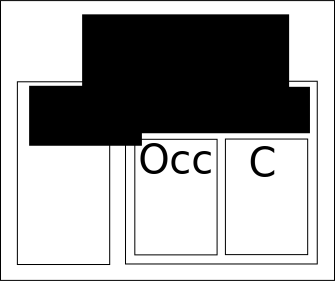
\includegraphics[width=6cm]{fm_index}
        \caption{Znázornenie štruktúry FM indexu}
        \label{fig:fm_index}
    \end{figure}
    
    \subsubsection{Komprimované sufixové pole}
    Komprimované sufixové pole (\emph{CSA - compressed suffix array}) pole sa využíva na zistenie pozície daného podreťazca v texte $T$. Nie je si ale potrebné držať v ňom pozície všetkých sufixov $T$, keďže pomocou \emph{LF mappingu} vieme zrekonštruovať podreťazec $T$ začínajúci na ľubovoľnej pozícii. Preto si stačí pamätať len pozície niektorých sufixov a potom pomocou \emph{LF mappingu} len čiastočne rekonštruovať $T$, pokým nedosiahneme nejakú pamätanú pozíciu sufixu. Komprimované sufixové pole zaberá iba zlomok pamäte oproti pôvodnému, no na oplátku sa kvôli nutnosti čiastočnej rekonštrukcie výrazne zvýši čas trvania operácie \emph{locate}.
    
    \subsubsection{Tabuľka prefixových súm}
    Táto tabuľka obsahuje pre každý znak $c$ danej abecedy počet výskytov lexikograficky menších znakov ako $c$ v danom reťazci $S$. Narozdiel od sufixového poľa ale nie je tak ľahko komprimovateľná, keďže frekvencie výskytu jednotlivých znakov sú na sebe navzájom nezávislé. Na druhej strane, zvyčajne býva veľkosť abecedy rádovo menšia než dĺžka textu, takže veľkosť tejto tabuľky bude prispievať do celkovej pamäťovej náročnosti len malou časťou\footnote{Špeciálne to platí v našom, bioinformatickom kontexte, kde používame štvorpísmenovú abecedu a genómy majú dĺžky v miliónoch.}.
    
    \subsubsection{Tabuľka výskytov}
    Tabuľka výskytov $Occ$ pre dané $c$ a $k$ vráti počet výskytov znaku $c$ v prefixe $S[0..k]$ daného reťazca $S$. Keď túto tabuľku skonštruujeme nad $BWT(T)$, tak \emph{LF mapping} vieme zadefinovať ako $$LF(i) = C[BWT(T)[i]] + Occ(BWT(T)[i], i)$$
    Rýchlosť prístupu k tejto tabuľke a jej pamäťová náročnosť je najdôležitejším faktorom FM indexu. 
    
    \bigskip
    
    Pre lepšiu predstavu uveďme príklad:
    
    \begin{example}
        \label{ex:fm_index}
        Nech $T = banana\$$, potom $BWT(T) = annb\$aa$. Tabuľky $C$ a $Occ$ skonštruované nad $BWT(T)$ potom vyzerajú nasledovne:
        
        \bigskip
        
        \begin{minipage}{2.5in}
            \begin{tabular}{ | c | c | c | c | c | }
                \multicolumn{5}{c}{\textbf{C pre \emph{annb\$aa}}} \\ \hline
                \textbf{c}    & \$ & a & b & n                     \\ \hline
                \textbf{C[c]} & 0  & 1 & 4 & 5                     \\ \hline
            \end{tabular}
        \end{minipage}
        \begin{minipage}{2.5in}
            \begin{tabular}{ | c | c | c | c | c | c | c | c | }
                \multicolumn{8}{c}{\textbf{Occ(c, k) pre \emph{annb\$aa}}} \\ \hline
                            & \textbf{a} & \textbf{n} & \textbf{n} & \textbf{b} & \textbf{\$} & \textbf{a} & \textbf{a} \\ \hline
                            & \textbf{0} & \textbf{1} & \textbf{2} & \textbf{3} & \textbf{4}  & \textbf{5} & \textbf{6} \\ \hline
                \textbf{\$} & 0          & 0          & 0          & 0          & 1           & 1 & 1 \\ \hline                 
                \textbf{a}  & 1          & 1          & 1          & 1          & 1           & 2 & 3 \\ \hline
                \textbf{b}  & 0          & 0          & 0          & 1          & 1           & 1 & 1 \\ \hline  
                \textbf{n}  & 0          & 1          & 2          & 2          & 2           & 2 & 2 \\ \hline
            \end{tabular}
        \end{minipage}
    \end{example}

    \subsection{Vyhľadávanie pomocou FM indexu}
    Vyhľadávanie v FM indexe rozdelíme na dve fázy - \emph{počítaciu} a \emph{lokalizačnú} (pri operácii \emph{count} stačí vykonať prvú časť, pre \emph{locate} obe). \emph{Počítacia} fáza má za úlohu identifikovať rozsah sufixov zo sufixového poľa, ktoré majú rovnaký prefix -- vyhľadávanú vzorku\footnote{Z definície sufixového poľa vyplýva, že sufixy s rovnakým prefixom nasledujú v sufixovom poli za sebou} a \emph{lokalizačná} fáza potom identifikuje vzorky v sufixovom poli.
    
    \subsubsection{Počítacia fáza}
    Hľadanie vzorky v sufixovom poli je časovo veľmi efektívne, pretože sa zároveň hľadajú všetky výskyty danej vzorky $P$ -- simultánnym posúvaním ukazovateľov hornej a dolnej hranice v sufixovom poli. Označme tieto ukazovatele $sp$ a $ep$ (z ang. \emph{starting} resp. \emph{ending pointer}). Znak $c$ bude obsahovať momentálne spracovávaný znak vzorky $P$, pričom začneme posledným znakom a budeme tiež využívať pomocné polia $Occ$ a $C$ zadefinované v predchádzajúcej časti. Ukazovateľ $sp$ bude inicializovaný na $C[c]$ a ukazovateľ $ep$ na $C[c + 1]$ -- v tomto prípade už tieto ukazovatele ukazujú na prvý resp. posledný výskyt posledného písmena $P$ v $F$\footnote{Pripomeňme, že $F$ je prvým stĺpcom $BWM$ a $F$ je vlastne pole znakov, ktoré zodpovedajú indexom sufixového poľa do pôvodného textu $T$.}.
    
    \bigskip
    
    \begin{pseudocode}[label=lst:fm_search_algorithm,caption={Algoritmus na hľadanie vzorky pomocou FM indexu}]
i = P.length - 1
c = P[i]
sp = C[c]
ep = C[c + 1]

while i > 0 do
  i = i - 1
  c = P[i]
  sp = C[c] + Occ(c, sp - 1)
  ep = C[c] + Occ(c, ep) - 1
end
    \end{pseudocode}
    
    $Occ(c, sp - 1)$ (riadok 5) vracia počet znakov $c$ v $BWT(T)[0..(sp - 1)]$. Keď k nemu pripočítame počet znakov, ktoré sú menšie než $c$ ($C[c]$) dostávame pozíciu prvého $c$ v rozsahu $sp$ až $ep$ v $F$. Operácie v riadkoch 5 a 6 realizujú \emph{LF mapping} pre prvý a posledný výskyt $c$ v $BWT(T)[sp..ep]$ (ak by sme nemali k dispozícii tabuľku $Occ$, museli by sme najprv nájsť prvý a posledný výskyt $c$ v $BWT(T)[sp..ep]$ a až potom použiť \emph{LF mapping}).
    
    \bigskip
    \begin{example}
        Postup vyhľadávania vzorky $P = nan$ by vyzeral nasledovne: \\ \\
        \begin{minipage}{2in}
            \begin{tabular}{ c c c }
                \multicolumn{3}{c}{\emph{P = na\textbf{n}}} \\
                \textbf{F} &        & \textbf{L} \\
                \$         & \ldots & a          \\            
                a          & \ldots & n          \\
                a          & \ldots & n          \\
                a          & \ldots & b          \\
                b          & \ldots & \$         \\
                \textbf{n} & \ldots & a          \\ 
                \textbf{n} & \ldots & a          \\
            \end{tabular}
        \end{minipage}
        \begin{minipage}{2in}
            \begin{tabular}{ c c c }
                \multicolumn{3}{c}{\emph{P = n\textbf{an}}} \\
                \textbf{F} &        & \textbf{L} \\
                \$         & \ldots & a          \\            
                a          & \ldots & n          \\
                \textbf{a} & \ldots & n          \\
                \textbf{a} & \ldots & b          \\
                b          & \ldots & \$         \\
                n          & \ldots & a          \\ 
                n          & \ldots & a          \\
            \end{tabular}
        \end{minipage}
        \begin{minipage}{2in}
            \begin{tabular}{ c c c }
                \multicolumn{3}{c}{\emph{P = \textbf{nan}}} \\
                \textbf{F} &        & \textbf{L} \\
                \$         & \ldots & a          \\            
                a          & \ldots & n          \\
                a          & \ldots & n          \\
                a          & \ldots & b          \\
                b          & \ldots & \$         \\
                \textbf{n} & \ldots & a          \\ 
                n          & \ldots & a          \\
            \end{tabular}
        \end{minipage}
    \end{example}
    \bigskip

    \subsubsection{Lokalizačná fáza}
    Výsledkom počítacej fázy sú dva indexy, $sp$ a $ep$, ktoré vymedzujú rozsah v sufixovom poli textu $T$. A práve prvky prvky v tomto rozsahu nám prezradia, na ktorých pozíciach textu $T$ nastala zhoda s vyhľadávanou vzorkou.
    
    \subsubsection{Časová zložitosť}
    Časová zložitosť počítacej fázy je lineárna vzhľadom na dĺžku hľadanej vzorky $P$, keďže v každej iterácii spracujeme jeden znak $P$. Na druhej strane, dĺžka textu $T$ na túto operáciu vplyv nemá, preto je táto metóda mimoriadne vhodná na spracovávanie dlhých textov, ako sú napríklad genómy. Zložitosť počítacej fázy je tiež nezávislá na počte výskytov vzorky v texte, keďže hľadáme len hornú a dolnú hranicu výskytu. V každej iterácii tiež spravíme dva dotazy do tabuľky $Occ$, takže výsledný čas závisí tiež lineárne od časovej zložitosti dotazov na $Occ$.
    
    Pri časovej zložitosti lokalizačnej fázy je situácia opačná -- nezávisí na dĺžke hľadanej vzorky, ale na počte výskytov, keďže pre každý jeden musíme pristúpiť ku sufixovému poľu. Preto o zložitosti rozhoduje implementácia sufixového poľa.
    
    \subsubsection{Zlepšenia}
    Ak by mala tabuľka $Occ$ odpovedať v konštantnom čase, zaberala by značné množstvo pamäte, preto sa v praxi pri jej implementácii používajú sofistikovanejšie dátové štruktúry ako napríklad \emph{wavelet tree} \cite{GGV03}.
    
    Čo sa týka lokalizačnej fázy, tak je potrebné spomenúť, že pamätanie si celého sufixového poľa by zaberalo priveľa pamäte, preto sa v praxi používajú napríklad komprimované sufixové pole -- ukladá sa len časť pôvodného sufixového poľa a chýbajúce hodnoty sa potom v prípade potreby dorátavajú pomocou pamätaných hodnôt.
    
    \todo{MTF, RL, wavelet, huffman, ... citacie, odkazy, fm index v2}
    
\section{Algoritmy na zostavovanie genómu}
    Výsledkom sekvenovania genómu (pri použití súčasných technológií) je veľké
    množstvo malých fragmentov - \emph{sequencing reads}, ktoré je potrebné
    zostaviť do jednej súvislej sekvencie. Náročnosť tejto úlohy závisí najmä
    od:
    
    \begin{itemize}
        \item dĺžky zostavovaného genómu - čím je kratší, tým je to jednoduchšie
        \item dĺžok jednotlivých fragmentov - čím sú dlhšie, tým lepsie
        \item priemernej hĺbky pokrytia - tzn koľko fragmentov v priemere
        pokrýva konkrétnu pozíciu zostavovanej sekvencie - čím viac, tým lepšie
    \end{itemize}

    \subsection{Najkratšie spoločné nadslovo}
    Asi najjednodušiu formuláciu problému zostavovania genómu predstavuje
    problém hľadania najkratšieho spoločného nadslova (\emph{shortest common
    superstring}).
    
    \begin{defn}
        Najkratším spoločným nadslovom reťazcov $S_1, S_2, \ldots, S_k$ nazývame
        najkratší reťazec $S$ taký, že každé $S_i$ je podslovo $S$.
    \end{defn}
    
    Tento problém je ale NP-ťažký, takže nepoznáme žiadny rýchly algoritmus,
    ktorý vždy nájde riešenie. Jednoduchá heuristika by vyzerala nasledovne:
    
    \begin{itemize}
        \item nájdi také dva fragmenty, ktoré majú najväčší prekryv, t.j.
        najdlhšiu $\alpha$ takú, že $S_i = \alpha\beta$ a $S_j = \gamma\alpha$
        \item spoj $S_i$ a $S_j$ do $\gamma\alpha\beta$
        \item opakuj prvý krok, kým neozostane iba jedno slovo
    \end{itemize}
    
    O tomto algorime sa dá dokázať, že je to 3.5-aproximačný algoritmus, t.j.
    nájdené riešenie bude mať vždy dĺžku nanajvýš 3.5-násobku optimálnej dĺžky.
    Síce je problém najkratšieho spoločného nadslova pomerne elegantnou
    formuláciou problému zostavovania genómov, je tento problém príliš ťažký na
    to, aby bolo jeho riešenie praktické pre veľké genómy. Preto sa v praxi
    používajú iné metódy.

    \subsection{Overlap-Layout-Consensus}
    Táto metóda, ako už jej názov naznačuje, pracuje v troch fázach:
    
    \subsubsection{Overlap}
    V tejto fáze assembler hľadá navzájom sa prekrývajúce fragmenty a spája ich do dlhších fragmentov, \emph{kontigov}. 
    
    Porovnávanie každej dvojice fragmentov by však bolo v praxi veľmi časovo náročné, nakoľko fragmentov môžu byť často milióny a pri porovnaní každej dvojice by sme potrebovali rádovo $O(n^2k)$ času (kde $n$ je počet fragmentov a $O(k)$ je čas, ktorý trvá porovnanie dvoch fragmentov). 
    
    Efektívnejšie algoritmy sú založené na predpoklade, že ak sa dva fragmenty úplne zhodujú na úseku dľžky aspoň $k$ (v praxi sa používa $k \approx 24$ ), tak pochádzajú z toho istého miesta v sekvenovanom genóme a teda sú spojené do jedného kontigu. 
    
    Vo všeobecnosti vyzerá tento postup nasledovne:
    \begin{itemize}
        \item vytvor zoznam podreťazcov dĺžky $k$ zo všetkých fragmentov, pričom ku každému podreťazcu si zapamätaj, z ktorého fragmentu pochádza
        \item lexikograficky utrieď zoznam podreťazcov
        \item skupiny výrazne sa prekrývajúcich fragmentov sa v utriedenom zozname budú vyskytovať pohromade a práve to sú dobrí kandidáti na spojenie do kontigov
    \end{itemize}
    
    \subsubsection{Layouy}
V druhej fáze assembler určuje relatívnu polohu jednotlivých kontigov a ich približné vzdialenosti, výsledné bloky kontigov sa nazývajú \emph{superkontigy}.

    \subsubsection{Consensus}
V poslednej fáze je vytvorená finálna sekvencia superkontigov, ktorá pokrýva genóm (alebo aspoň jeho časti). 
\\ \\
Často sa ale zvykne používať aj grafová reprezentácia tohto algoritmu. Vrcholmi grafu sú fragmenty, hrana medzi vrcholmi je vtedy, ak sa tieto dva fragmenty prekrývajú (overlap). V layout fáze sa tento graf zjednodušuje (napr. vymazanie nadbytočných hrán). Fáza consensus potom spočíva v nájdení hamiltonovskej cesty v tomto grafe.
    
    \subsection{De Bruijnove grafy}
    Tento prístup využíva to, že (obvykle) máme pri sekvenovaní veľké množstvo
    dát, a preto si môžme dovoliť časť obsiahnutej informácie v nich
    odignorovať.
    
    Pre jednoduchosť budeme predpokladať, že všetky fragmenty pochádzajú z
    jedného vlákna a snažíme sa zostaviť len jeden, úplne pokrytý chromozóm.

    Algoritmus pre vytvorenie \emph{de Bruijnovho grafu} vyzerá nasledovne:
    
    \begin{itemize}
        \item vytvor zoznam všetkých podreťazcov dĺžky $k$ zo všetkých
        fragmentov ($k$-tice)
        \item vrcholy grafu budú tvoriť všetky úseky dĺžky $k - 1$ (teda
        podreťazce podreťazcov dĺžky $k$)
        \item jednotlivé $k$-tice budú reprezentované orientovanými hranami v
        grafe, pričom $k$-tica $s_1 s_2 \ldots s_k$ spája vrcholy $s_1 s_2
        \ldots s_{k-1}$ a $s_2 s_3 \ldots s_k$. 
    \end{itemize}
    
    Eulerovský ťah v takomto grafe potom predstavuje hľadaný genóm.
    
    \begin{example}
        Uvažujme fragmenty \texttt{CCTGCC} a \texttt{GCCACC} a $k = 3$. Zoznam
        $k$-tic teda bude vyzerať nasledovne:
        
        \bigskip
        
        \begin{tabular}{ c c }
            \textbf{CCTGCC} & \textbf{GCCACC} \\  
            \texttt{CCT}    & \texttt{GCC}    \\
            \texttt{CTG}    & \texttt{CCA}    \\
            \texttt{TGC}    & \texttt{CAC}    \\
            \texttt{GCC}    & \texttt{ACC}    \\
        \end{tabular}  
        
        \bigskip
        
        Úseky dĺžky $k-1$: \texttt{CC}, \texttt{CT}, \texttt{TG}, \texttt{GC},
        \texttt{CA}, \texttt{AA}, \texttt{AC}
        
        \bigskip
        
        Graf: 
        
        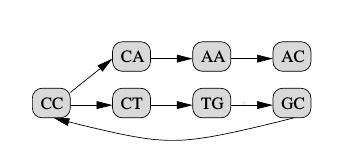
\includegraphics{graf.png}
    \end{example}
            
    \chapter{Problém indexovania readov}
        \label{ch:problem_indexovania_readov}
        \todo{bioinformaticka motivacia problemu. blabla. bioinf definicia problemu. Vo
svojej praci sa Dr. Peter Boza PhD., CSc., PanVesmiru, zaobera \ldots, kde
riesi \ldots a odtial pochadza motivacia riesit problem \ldots.}

\section{Definícia problému}

Úlohou bude teda vytvoriť efektívnu dátovú štruktúru, ktorá načíta veľkú sadu
relatívne krátkych reťazcov (\emph{sequence reads}) a umožní dostatočne rýchlo
odpovedať na dotaz (\emph{query}) \emph{,,vráť tie reťazce, ktoré obsahujú ako
podreťazec reťazec $P$``}, pričom dĺžka reťazca $P$ je dopredu daná. Dôraz
budeme klásť ako na rýchlosť odpovedania na query, tak aj na pamäťovú
efektívnosť tejto dátovej štruktúry. Formálne:

\begin{description}
    \item[Vstup] \hfill \\
        Na vstupe pre konštrukciu dátovej štruktúry sú $k, n, L \in N$ a množina
        $R$ taká, že:
        $$R = \{r_0, r_1, \ldots, r_{n-1} :
        \forall i : 0 \leq i < n : |r_i| = L \wedge \forall j : 0 \leq
        j < L : r[j] \in \Sigma \}$$ kde $|\Sigma| = 4$.
    \item[Výstup] \hfill \\
        Výstupom pre dotaz $P$, kde $$|P| = k \wedge \forall i : 0 \leq i < k :
        P[i] \in \Sigma$$ je taká množina $O$, že: 
        $$O = \{r_m, r_{m+1}, \ldots, r_{m+l} : \forall i : m \leq i \leq m +
        l : r_i \in R \wedge issubstring(P, r_i) \}$$ pričom predikát
        $issubstring$ je definovaný ako $$issubstring(p, S) \leftarrow \exists i
        \in N: 0 \leq i < |S| - |p| + 1 : \forall j : 0 \leq j < |p| : p[j] ==
        S[i+j] $$        
\end{description}

Takto zadaná úloha je ale veľmi nekonkrétna a vo všeobecnosti ťažko riešiteľná.
Avšak to, že tento problém budeme riešiť v bioinformatickom kontexte nám úlohu
uľahčí:

\begin{itemize}
    \item Vieme, že všetky \emph{sequence reads} $r_i$ pochádzajú z nejakého
    spoločného nadslova (sekvenovanej DNA), pričom pri sekvenovaní mohla s
    istou pravdepodobnosťou nastať chyba. \todo{odkaz na definiciu chyby
    sekvenovania}. Pravdepodobnosť chyby budeme uvažovať na úrovni $0.1\% - 2\% $.
    \item Dĺžka spoločného nadslova sa pohybuje medzi $10^6$ (dĺžka genómu
    baktérií je niekde na úrovni $4 \cdot 10^6$) a $10^9$ (dĺžka genómu človeka
    je asi $3 \cdot 10^9$).
    \item Dĺžky \emph{readov} $l$ sa pohybujú v rozmedzí $100 - 150$
    \item Pri sekvenovaní sa využíva miera pokrytia (\todo{odkaz na definiciu
    miery pokrytia}) v rozmedzí $10\times$ až $100\times$, z čoho nám v
    kombinácii s dlžkou spoločného nadslova a dlžkou \emph{readov} vychádza
    obmedzenie pre počet \emph{readov} na vstupe na 
    $n \in [ 10^5, \frac{2}{3} \cdot 10^9 ]$ \todo{ugh. toto nie je privela?}
    \item Dĺžku podreťazca $P$ budeme uvažovať v rozmedzí $13 -15$. 
    \item Jemná modifikácia predikátu $issubstring(p, S)$: $$issubstring2
    \leftarrow issubstring(p, S) \vee issubstring(p, revcompl(S))$$ kde
    $revcompl(S)$ je funkcia, ktorá pre vstupný reťazec $S$ vráti jeho reverzný
    komplement (\todo{odkaz na definiciu reverzneho komplementu})
\end{itemize}

Cieľom bude dosiahnuť čo najnižsiu pamäťovú zložitosť, pri zachovaní
,,rozumnej`` časovej zložitosti. Očakávaná pamáťová zložitosť bude teda $O(n +
s)$, kde $n$ je počet načítaných \emph{readov} a $s$ je dĺžka spoločného
nadslova. (Triviálnym riešením by bolo $O(n \cdot L)$, kde $L$ je dĺžka
\emph{readu})

\section{Riešenie s použitím hash mapy}

\section{Riešenie s použitím GkArray}

\section{Porovnanie}
        
    \chapter{CR-index}
        V tejto kapitole predstavíme naše riešenie \emph{problému indexovania readov} -- dátovú štruktúru \emph{CR-index} (z eng. \emph{Compressed Read index}), ktorá je navrhnutá tak, aby sa vyhla nedostatkom, ktorými trpia riešenia s použitím \emph{GkArray} alebo hash mapy. Pripomeňme, že úlohou tejto dátovej štruktúry bude efektívne (najmä vzhľadom na pamäť) zaindexovať veľkú sadu relatívne krátkych reťazcov nad malou abecedou -- \emph{sequence readov} -- a má vedieť odpovedať na dotaz \emph{,,vráť mi všetky ready také, že obsahujú $p$ ako podreťazec``}.

\section{Princíp fungovania}

\subsection{Komprimácia vstupu}
Kým \emph{GkArray} ready zo vstupu iba zreťazil a nad týmto dlhým reťazcom potom budoval sufixové polia a ostatné pomocné štruktúry, hlavnou myšlienkou \emph{CR-indexu} je, ako už napovedá názov, ready najprv vhodným spôsobom skomprimovať a až potom ďalej spracovávať. Využijeme to, že reťazce, ktoré máme za úlohu indexovať majú čosi spoločné -- vznikli sekvenovaním jedného genómu. Keďže pokrytie sa pri sekvenovaní zvyčajne pohybuje na úrovni $10\times$ -- $100\times$, znamená to, že ready obsahujú veľké množstvo nadbytočných informácií. Pomocou nejakého assembleru čiastočne zrekonštruujeme pôvodný genóm -- čiastočne preto, lebo výstupom assemblerov pre nejakú sadu readov nebýva vo všeobecnosti súvislý genóm, ale len sada kontigov resp. superkontig. Tiež nemáme zaručené, že každý read zo vstupu sa v niektorom kontigu musí nachádzať. Tieto chýbajúce ready potom musíme efektívne nájsť a nejakým spôsobom pridať ku kontigom, aby sme neprišli o žiadnu informáciu.

Pre začiatok predpokladajme, že ready na vstupe sú bez sekvenovacích chýb -- to znamená, že pre každý read platí, že je podreťazcom pôvodného genómu, ktorý bol sekvenovaný. Assembler by mal byť pri rekonštruovaní genómu pomerne úspešný (samozrejme ak majú ready dostatočné pokrytie) a relatívne málo readov by malo chýbať medzi kontigmi. V tomto prípade by sme teda spolu zreťazili kontigy a všetky chýbajúce ready -- tým dostaneme bezstratovo komprimovaný vstup. Ako ale nájdeme ready, ktoré nie sú podreťazcom zreťazenia kontigov? Jednoducho -- nad zreťazením kontigov skonštruujeme FM-index, ktorého sa postupne budeme pýtať na všetky ready zo vstupu (a ich reverzné komplementy) a v prípade, že FM-index tento read (ani jeho reverzný komplement) nenájde, označíme ho ako chýbajúci.

Výsledkom komprimačnej fázy je teda zreťazenie kontigov a readov zo vstupu, ktoré nie sú podreťazcom zreťazenia kontigov a ani ich reverzný komplement nie je podreťazcom zreťazenia kontigov. Tento dlhý reťazec nazveme \emph{superstring} (neskôr ho definujeme aj formálne).

Superstring v princípe predstavuje najkratšie spoločné nadslovo pre ready, no keďže hľadanie najkratšieho spoločného nadslova je NP-úplný problém, musíme sa uchýliť ku vhodnej aproximácii, čo za nás spraví assembler.

\subsection{Index}
\label{ssec:index}
V ďalšej fáze konštrukcie CR-indexu vytvoríme nad superstringom (opäť) FM-index. V tejto chvíli sme už schopní efektívne vyhľadávať vzorky v superstringu, no keď nám operácia FM-indexu \emph{locate} vráti zoznam pozícií superstringu, kde sa daná vzorka nachádza, nevieme z toho povedať ktorým readom tieto pozície prislúchajú. Potrebujeme si teda predrátať, kde sa ktorý read nachádza. Na to použijeme pole \emph{positions} -- jeho prvkami budú trojice $(i, r, b)$ - $i$ bude označovať index v superstringu, kde začína read $r$. Logická premenná $b$ označuje, či sa v superstringu nachádza samotný read ($b=0$) alebo jeho reverzný komplement ($b=1$). Algoritmus na konštrukciu CR-indexu teda vyzerá nasledovne\footnote{Táto implementácia slúži len pre účely vysvetlenia konštrukcie CR-indexu. Reálna implementácia vyzerá trochu odlišne a popíšeme ju v kapitole \ref{ch:implementacia}.}:

\bigskip
\begin{pseudocode}[label=lst:cr_index_construction,caption={Algoritmus konštrukcie CR-indexu nad readmi bez chýb.}]
assembler = Assembler.new <* \label{lst:cr_index_construction_assembler} *>
superstring = ""
positions = Array.new

contigs = assembler.assemble(R) <* \label{lst:cr_index_construction_assemble} *>
foreach c : contigs do <* \label{lst:cr_index_construction_contigs_start} *>
  superstring += c 
end <* \label{lst:cr_index_construction_contigs_end} *>

contigs_fm_index = FMIndex.new(joint_contigs) <* \label{lst:cr_index_construction_fm_index} *>

foreach r : R  do
  matches = contigs_fm_index.locate(r) <* \label{lst:cr_index_construction_locate} *>
  matches2 = contigs_fm_index.locate(rev_compl(r)) <* \label{lst:cr_index_construction_rev_compl} *>

  if matches.size() == 0 && matches2.size() 
    positions.push(superstring.length(), r, 0) <* \label{lst:cr_index_construction_push} *> 
    superstring += r <* \label{lst:cr_index_construction_superstring_r} *>  
  else
    foreach m : matches do
      positions.push([m, r, 0]) <* \label{lst:cr_index_construction_push2} *>  
    end
    
    foreach m : matches2 do
      positions.push([m, r, 1]) <* \label{lst:cr_index_construction_push3} *>  
    end
  end
end

positions.sort <* \label{lst:cr_index_construction_sort} *>  
fm_index = FMIndex.new(superstring) <* \label{lst:cr_index_construction_fm_index2} *>
\end{pseudocode}
\bigskip

Premenná $R$ označuje množinu readov, ktorú máme na vstupe. Objekt \emph{assembler} (riadok \ref{lst:cr_index_construction_assembler}) predstavuje zapuzdrenie volania vhodného assemblera, jeho metóda \emph{assemble} (riadok \ref{lst:cr_index_construction_assemble}) vracia pre pole readov na vstupe pole reťazcov predstavujúcich kontigy, ktoré assembler poskladal z readov. Objekt \emph{FM-index} (riadok \ref{lst:cr_index_construction_fm_index}) je vhodná implementácia FM-indexu podporujúca operáciu \emph{locate} (viď. kapitolu \ref{sec:fm_index}), ktorá pre vzorku na vstupe vráti pole indexov reťazca nad ktorým je tento FM-index skonštruovaný, na ktorých daná vzorka začína. Funkcia \emph{rev\_compl(s)} (riadok \ref{lst:cr_index_construction_rev_compl}) vracia pre reťazec na vstupe jeho reverzný komplement (podľa definície \ref{def:reverzny_komplement}).

Algoritmus najprv zavolá assembler (riadok \ref{lst:cr_index_construction_assemble}), pomocou ktorého vytvorí kontigy, ktoré zreťazí (riadky \ref{lst:cr_index_construction_contigs_start} -- \ref{lst:cr_index_construction_contigs_end}). Potom prebehne konštrukcia pomocného FM-indexu (riadok \ref{lst:cr_index_construction_fm_index}) nad zreťazenými kontigmi. Následne sa pre každý read $r$ a jeho reverzný komplement zavoláme metódu \emph{locate} tohto FM-indexu (riadky \ref{lst:cr_index_construction_locate} -- \ref{lst:cr_index_construction_rev_compl}). Ak sa ani jeden z nich v superstringu nenachádza, tak ho tam pridáme (riadok \ref{lst:cr_index_construction_superstring_r}). Už predtým už ale vieme, na akej pozícii bude tento read v superstringu začínať (keďže ho pridávame na koniec) a môžeme túto informáciu vložiť do poľa \emph{positions} (riadok \ref{lst:cr_index_construction_push}). Pre ready, ktoré sa v superstringu nachádzajú pridáme do poľa \emph{positions} informáciu o ich výskytoch (riadok \ref{lst:cr_index_construction_push2}) resp. výskytoch ich reverzných komplementov (riadok \ref{lst:cr_index_construction_push3}). Pole \emph{positions} nakoniec utriedime (riadok \ref{lst:cr_index_construction_sort}) -- ako uvidíme v ďalšej časti, pomôže nám to rýchlejšie identifikovať ready obsahujúce hľadanú vzorku. Nad superstringom, ktorý sme úspešne zreťazili so všetkými chýbajúcimi readmi potom skonštruujeme nový FM-index (riadok \ref{lst:cr_index_construction_fm_index2}). Práve ten spolu s poľom \emph{positions} predstavujú výstup konštrukcie celého CR-indexu.

\subsection{Dotazy}
Úlohou je pre reťazec $p$ na vstupe vrátiť tie ready, ktoré obsahujú $p$ ako podreťazec. Najprv uvedieme algoritmus v pseudokóde a potom ho vysvetlíme:

\bigskip
\begin{pseudocode}[label=lst:cr_index_query,caption={Algoritmus dotazu \emph{locate} CR-indexu nad readmi bez chýb.}]
def locate(p)
  retval = Array.new
  indexes = fm_index.locate(p) <* \label{lst:cr_index_query_locate} *>  
  
  foreach i : indexes do <* \label{lst:cr_index_query_foreach} *>  
    start_index = [i + k - l, -1, 0] <* \label{lst:cr_index_query_start_index} *>  
    end_index = [i, INT_MAX, 1] <* \label{lst:cr_index_query_end_index} *>  
    
    low = positions.lower_bound(start_index) <* \label{lst:cr_index_query_low} *>  
    up = positions.upper_bound(end_index) <* \label{lst:cr_index_query_up} *>  
    
    for (pos = low; pos != up; pos++) do <* \label{lst:cr_index_query_foreach2} *>
      if (pos[2] == 0)
        retval.push(pos[1]) <* \label{lst:cr_index_query_push_read} *>
      else
        retval.push(rev_compl(pos[1])) <* \label{lst:cr_index_query_push_rev_compl} *>
      end
    end
  end
  
  return retval
end
\end{pseudocode}
\bigskip

Premenné $fm\_index$ a $positions$ sú výsledkom konštrukcie z časti \ref{ssec:index}, premenná $l$ predstavuje dĺžku každého readu, premenná $k$ má hodnotu dĺžky dotazu (podľa toho, ako sme problém \emph{indexovania readov} zadefinovali v časti \ref{sec:definicia_problemu} máme obe hodnoty k dispozícii na vstupe pri konštrukcii CR-indexu, t.j. predstavujú parametre konštrukcie) a konštanta $INT\_MAX$ je najväčšia hodnota pre celočíselný dátový typ.

V prvom kroku vyhľadáme výskyty $p$ v superstringu pomocou FM-indexu (riadok \ref{lst:cr_index_query_locate}), ktorý sme skonštruovali počas predchádzajúcej fázy -- výsledkom bude zoznam pozícií v superstringu, kde bola vzorka $p$ nájdená. Následne potrebujeme tieto pozície preložiť na ready, ktorým prislúchajú a na to využijeme pole \emph{positions}. To spravíme tak, že v ňom pre každý index $i$ (riadok \ref{lst:cr_index_query_foreach}) pomocou binárneho vyhľadávania obmedzíme rozsah, kde sa nachádzajú relevantné hodnoty -- tie prvky, ktoré označujú začiatky readov, ktoré obsahujú ako podreťazec tento výskyt hľadanej vzorky. Práve tu využijeme to, že toto pole je utriedené podľa prvej súradnice -- indexu ukazujúceho na pozíciu v superstringu. Metódy $lower\_bound$\footnote{Podľa \url{http://www.cplusplus.com/reference/algorithm/lower_bound/}} (riadok \ref{lst:cr_index_query_low}) resp. $upper\_bound$ (riadok \ref{lst:cr_index_query_up}) vrátia takú pozíciu v poli, že hodnota na tejto pozícii nie je menšia resp. je väčšia ako $start\_index$ resp. $end\_index$. Pre $start\_index$ preto zvolíme hodnotu, ktorá popisuje najľavejší index v superstringu taký, že read na ňom začínajúci môže obsahovať výskyt vzorky $p$ začínajúci na indexe $i$ (pre $end\_index$ analogicky najpravejší read. Viď príklad \ref{ex:najlavejsi_najpravejsi_read}). Všetky takto ohraničené hodnoty poľa \emph{positions} (riadok \ref{lst:cr_index_query_foreach2}) predstavujú ready, ktoré obsahujú tento výskyt vzorky $p$ -- posledné, čo ostáva je pridať do výstupného poľa \emph{retval} tento read (riadok \ref{lst:cr_index_query_push_read}) resp. jeho reverzný komplement (riadok \ref{lst:cr_index_query_push_rev_compl}) -- podľa toho, ktorý z nich je v superstringu uložený (a indikátor toho sme si pri konštrukcii poľa \emph{positions} uložili ako tretiu hodnotu pre každý prvok). Metóda \emph{locate} teda pre hľadanú vzorku $p$ vráti zoznam readov, ktoré ju obsahujú ako podreťazec. Pre splnenie poslednej podmienky z časti \ref{sec:definicia_problemu} by sme pre dotaz na vzorku $p$ mali zavolať metódu \emph{locate} aj pre vstup $rev\_compl(p)$ a výstupy pre obe volania spojiť do jedného poľa a vrátiť ako výstup to.

\bigskip
\begin{example}
\label{ex:najlavejsi_najpravejsi_read}
Ilustrácia toho, ako by mohol vyzerať najľavejší a najpravejší read v superstringu pre vzorku $p=GTCG$, $k=3$, $l=10$. Ak vzorka $p$ začína v superstringu na indexe $i$, tak najľavejší read začína na indexe $i+k-l$ a najpravejší na indexe $i$.

$$
  ss=
  \ldots
  ACTTG
  \rlap{$\overbracket{\phantom{ATACCG              \mathbf{GTCG}}}^{read 1}$}
                               ATACCG\underbracket{\mathbf{GTCG}             AAAAAA}_{read 2}
  GGTC
  \ldots
$$
\end{example}
\bigskip

\begin{example}
Uvažujme sadu readov $R=\{AAATTG, AATTGG, ATTGGC, GCCCAA,\\ CCCATA, $ $GGTAAT, GTAATC, TAATCA, ATCAAA\}$, kde $l=6$ a $p=4$. Ďalej predpokladajme, že výstupom assemblera sú kontigy $c_0=AAATTGGCCCAA$ \\ a $c_1=TTGATTACC$. Ich zreťazením a doplnením chýbajúcich reťazcov dostávame nasledovný superstring: \\
$$
  ss=
  \overbracket{AAATTGGCCCAA}^{c_1}
  \underbracket{TTGATTACC}_{c_2}
  \overbracket{CCCATA}^{r_3}
  \underbracket{ATCAAA}_{r_7}
$$
Pole \emph{positions} potom vyzerá nasledovne:

\begin{center}
    \begin{tabular}{ | c | c | c | }
        \hline
        \textbf{i} & \textbf{read} & \textbf{rev\_compl?} \\ \hline
        0  & AAATTG & 0 \\ \hline
        1  & AATTGG & 0 \\ \hline
        2  & ATTGGC & 0 \\ \hline
        6  & GCCCAA & 0 \\ \hline
        13 & TAATCA & 1 \\ \hline
        14 & GTAATC & 1 \\ \hline
        15 & GGTAAT & 1 \\ \hline
        21 & CCCATA & 0 \\ \hline
        27 & ATCAAA & 0 \\ \hline
    \end{tabular}
\end{center}
\bigskip

Ilustrujme dotaz pre vzorku $p=AAT$:
$$
A\mathbf{AAT}TGGCCCAATTGATTACCCCCAT\mathbf{AAT}CAAA
$$
Vidíme, že FM-index nad superstringom nám ako výsledok vrátil dve hodnoty -- 1 a 26. Ak $i=1$, potom začiatok najľavejšieho readu, ktorý môže vzorku obsahovať je 0, začiatok najpravejšieho 1, iterátor \emph{low} (riadok \ref{lst:cr_index_query_low} listingu \ref{lst:cr_index_query}) ukazuje na index 0 poľa \emph{positions} a iterátor \emph{up} (riadok \ref{lst:cr_index_query_up}) na pozíciu 2 (túto hodnotu už iterátor \emph{pos} pri iterovaní (riadok \ref{lst:cr_index_query_foreach2}) nenabudne). Výsledkom teda budú ready začínajúce na indexoch 0 a 1 -- $AAATTG$ a $AATTGG$.

Pokračujme pre $i=26$. Iterátor \emph{low} bude ukazovať na index 8 v poli \emph{positions} (lebo najľavejší read obsahujúci tento výsky vzorky $p$ môže začínať na indexe 23). Iterátor \emph{up} bude ukazovať tiež na index 8, takže cyklus \emph{for} na riadku \ref{lst:cr_index_query_foreach2} sa nevykoná ani raz -- čo je v poriadku, keďže síce sme našli výskyt vzorky v superstringu, no nachádzal sa akurát na rozhraní readov a teda ani jeden read ho neobsahoval.

V tomto momente je dôležité si všimnúť, že týmto spôsobom sme nenašli všetky výskyty vzorky $p=AAT$, napríklad read $GGTAAT$ ju obsahuje, no tento read sme (zatiaľ) na výstup neposunuli. Assemblery totiž pokladajú ready a ich reverzné komplementy za identické a teda sa môže stať, že niektorý kontig bude zložený len z reverzných komplementov -- v našom príklade je to $c_1$. Preto pri zisťovaní výskytu vzorky $p$ potrebujeme vykonať dopyt aj pre $rev\_compl(p)$ a výsledné množinu readov zjednotiť. Pre vzorku $TAA = rev\_compl(AAT)$ nám už FM-index vráti výskyty v superstringu, ktoré potom úspešne preložíme na chýbajúce ready.

Je nutné poznamenať, že realizáciou dotazovania týmto spôsobom vrátime aj ready, ktoré obsahujú reverzný komplement vzorky $p$ -- predstavme si, že by sme robili dotaz pre $p=TACC$, v tom prípade vrátime na výstup aj read $GGTAAT$, ktorý túto vzorku neobsahuje. To je ale v poriadku, keďže to súhlasí s našou definíciou \emph{problému indexovania readov} (viď poslednú odrážku v časti \ref{sec:definicia_problemu}).

\end{example}

\section{Ready s chybami}
\label{sec:ready_s_chybami}
Bohužiaľ, zjednodušením situácie vo forme popierania existencie sekvenovacích chýb sa až príliš vzďaľujeme realite. Ako sa teda zmení situácia, ak máme brať do úvahy, že v readoch sa vyskytujú chyby?

Pripomeňme, že pri probléme \emph{indexovania readov} tak, ako sme ho zadefinovali v kapitole \ref{ch:problem_indexovania_readov} uvažujeme len substitučné chyby -- čo znamená, že read sa môže v niektorých bázach líšiť od svojho ,,obrazu`` v pôvodnom genóme.

V prvom rade assembler nebude pri konštrukcii kontigov ani zďaleka tak úspešný ako v predchádzajúcom prípade -- chyby budú znižovať pravdepodobnosť, že úspešne odhalí prekryvy medzi readmi, ciže výstupom assembleru budú oveľa kratšie kontigy, čiže aj ,,kompresný pomer`` bude výrazne nižší a to viac readov bude potrebné pripojiť na koniec. Ak si uvedomíme, že pri indexovaní readov napríklad s dĺžkou 100 báz a chybovosťou $1\%$ má takmer každý read aspoň jednu chybu, vidíme, že tento spôsob indexovania je pre ready s chybami nepostačujúci a komprimáciu vstupu je potrebné robiť sofistikovanejšie.

,,Komprimovateľnosť`` readov zvýšime tak, že pred tým, ako ich dostane assembler na vstup budú opravené -- korekcia readov (\emph{sequencing read correction}) je známy problém, na ktorý existuje množstvo riešení. \todo{sem by sa hodili nejake citacie} Čo nám ale skomplikuje situáciu je fakt, že kontigy budú obsahovať opravené ready a nie originálne, ktoré sme dostali na vstupe -- preto si budeme musieť pamätať aj ďalšie informácie týkajúce sa aplikovaných korekcií, aby sme vedeli prevádzať transformácie medzi opravenými a neopravenými readmi. Tým sme však stále nevyriešili situáciu, čo s chýbajúcimi readmi. Ak by sme v zreťazených kontigoch hľadali pôvodné, neopravené ready, chýbalo by ich, pochopiteľne, veľmi veľa a tým pádom by komprimácia nebola tak úspešná. Zvoľme opačný prístup -- v zreťazených kontigoch budeme hľadať opravené ready a tie, ktoré v kontigoch nie sú obsiahnuté zreťazíme na koniec. Zamyslime sa teraz, ako by prebiehal dotaz -- ak existuje výsky vzorky $p$ v superstringu, znamená to, že nejaký \emph{opravený} read obsahuje hľadanú vzorku. To ale neznamená, že ju obsahoval aj pôvodný read -- našťastie túto situáciu vieme ľahko vyriešiť pomocou zapamätaných korekcií -- k danému opravenému readu skonštruujeme pôvodný a v ňom overíme, či je $p$ jeho podreťazcom. Týmto spôsobom vieme vylúčiť \emph{false positives}. Problematickejšie to bude z druhej strany -- vieme ale takto nájsť \emph{všetky} výskyty vzorky $p$ medzi pôvodnými readmi? Uvažujme nasledovný príklad:

\begin{example}
Uvažujme sadu readov\footnote{Táto sada readov je zámerne extrémne jednoduchá, našim cieľom je len ilustrovať princíp problému} $R=\{AAAAACCC, TAAAACCC, AAAACCCC,$ \\ $ AAGACCCG, CCCCTGTG\}$, kde $l=8$ a $p=6$. Nech korekcie readov vyzerajú nasledovne:

\begin{align*}
AAAAACCC \rightarrow AAAAACCC \\
\mathbf{T}AAAACCC \rightarrow \mathbf{A}AAAACCC \\
AAAACCCC \rightarrow AAAACCCC \\
AA \mathbf{G} ACCC \mathbf{G} \rightarrow AA \mathbf{A} ACCC \mathbf{C} \\
CCC \mathbf{T} TGTG \rightarrow CCC \mathbf{C} TGTG
\end{align*}

Ďalej predpokladajme, že výstupom assemblera spusteného nad opravenými readmi je jeden kontig $c_0=AAAAACCCC$. Po doplnení chýbajúcich \emph{opravených} readov je výstupom superstring $ss=AAAAACCCCCCCCTGTG$. Zamyslime sa teraz, ako by vyzeral dotaz na vzorku $p=TAAAAC$ -- tá sa nachádza v pôvodnom reade $TAAAACCC$, no v superstringu sa už nevyskytuje. Možnosťou by bolo skúsiť vyhľadať všetky vzorky líšiace sa oproti $p$ v jednom znaku, akoby simulovať opravu chyby readu aj vo vzorke. Tým nám lineárne narastie počet dotazov na FM-index nad superstringom. Ak by sme hľadali vzorku $p=GACCCG$ (nachádza sa v pôvodnom reade $AAGACCCG$), potrebovali by sme hľadať ďalej -- výskyt tejto vzorky v pôvodnom reade postihli až dve korekcie. Ak by sme mali vygenerovať všetky možné vzorky líšiace sa od pôvodnej na dvoch miestach, je ich už kvadraticky veľa. Vyzerá to teda, že ani tento prístup, použiť len opravené ready, nebude sláviť úspech. Problematické vyzerajú byť tie ready, v ktorých sú pozície opráv príliš blízko seba -- tak, že by mohli ,,zasiahnúť`` vzorku, t.j. sú bližšie ako $p$.
\end{example}

V konečnom dôsledku teda vidno, že vhodný prístup leží kdesi uprostred možností zreťaziť s kontigmi (nad opravenými readmi) povodné a opravené ready -- budeme sa musieť vhodne vysporiadať s readmi, ktoré majú korekcie ,,príliš blízko seba``.

\section{Navrhovaná implementácia}
V predchádzajúcich častiach sme pojem superstring používali dosť voľne, teraz ho konečne riadne zadefinujeme. Predtým ale ešte uvedieme niektoré označenia a definície.

\subsection{Definície a označenia}

\subsubsection{Substitučná editačná vzdialenosť}
\begin{defn}
Substitučnú editačnú vzdialenosť dvoch reťazcov s a t rovnakej dĺžky l definujeme nasledovne:
$$
edt_s(s, t) = \left\vert{ \{~i~|~0 \leq i < l~\land s[i] \neq t[i] ~\} }\right\vert
$$
\end{defn}

Inými slovami, pre dva rovnako dlhé reťazce je to počet pozícií, na ktorých sa líšia.

\begin{example}
$edt_s(ACCTGG, TCCTGC) = 2$ 
\end{example}

\subsubsection{Superstring}
\begin{defn}
Superstringom množiny reťazcov R rovnakej dĺžky l s parametrom p~$\in \mathbb{N}$ označujeme taký reťazec S, pre ktorý platí, že každý reťazec $r \in R$ spĺňa aspoň jednu z nasledujúcich podmienok:
    \begin{enumerate}[(a)]
    \item r je podreťazcom S
    \item rev\_compl(r) je podreťazcom S
    \item existuje podreťazec s reťazca S s dĺžkou l taký, že 
    $$
    \forall i : 0 \leq i \leq l - p : edt_s(r[i, i+p-1], s[i, i+p-1]) \leq 1
    $$
    \item existuje podreťazec s reťazca S s dĺžkou l taký, že 
    $$
    \forall i : 0 \leq i \leq l - p : edt_s(rev\_compl(r)[i, i+p-1], s[i, i+p-1]) \leq 1
    $$    
    \end{enumerate}
\end{defn}

Povedané inak, superstringom množiny reťazcov $R$ je taký reťazec, v ktorom pre každý reťazec $r$ z $R$ platí, že buď on alebo jeho reverzný komplement je podreťazcom superstringu alebo pre $r$ alebo jeho reverzný komplement vieme nájsť podreťazec superstringu rovnakej dĺžky, ktorý sa od $r$ (resp. jeho reverzného komplementu) ,,líši len tu a tam`` -- to znamená, že indexy, na ktorých majú tieto dva reťazce rôzne znaky nie sú ,,príliš`` blízko seba, t.j. každé dva sú od seba vzdialené aspoň $p$.

\subsection{Korekcia readov}
% zadefinovat korekcnu funkciu, ta je nad R, Correcter ju potom realizuje
\begin{ozn}
Označme ako $corr_R(r)$ \emph{korekčnú} funkciu nad množinou readov $R$, ktorej výstupom pre read $r$ je opravený read $r_{corr}$, čo je read rovnakej dĺžky, ktorý sa môže (ale nie nutne musí) líšiť od pôvodného readu na niektorých pozíciach.
\end{ozn}

Fáza korekcie readov bude prebiehať tak, že ako prvé vygenerujeme sadu opravených readov. Potom skonštruujeme pole \emph{diff} a nakoniec rozdelíme ready na dve skupiny, ako uvidíme neskôr.

\subsubsection{Pole diff}
Pole \emph{diff} skonštruujeme tak, aby obsahovalo informácie o aplikovaných korekciách na jednotlivé ready. Formálne by sme ho definovali ako:

\begin{defn}
Množinu korekcií pre množinu readov $R$ a korekčnú funkciu $corr_R$ definujeme ako 
$$
diff = \{(corr_R(r), i, r[i])~|~\forall r \in R~\forall i : 0 \leq i < |r| : corr_R(r)[i] \neq r[i] \}
$$
\end{defn}

Algoritmus na konštrukciu poľa \emph{diff} by vyzeral nasledovne:

\bigskip
\begin{pseudocode}[label=lst:cr_index_diff_construction,caption={Algoritmus konštrukcie poľa diff.}]
diff = Array.new
correcter = Correcter.new <* \label{lst:cr_index_diff_construction_correcter} *>
corrected_reads = correcter.correct_reads(R)

for (i = 0; i < R.length; i++) do
  for (j = 0; j < R[i].length; j++) do
    if R[i][j] != corrected_reads[i][j]
      diff.push([corrected_reads[i], j, R[j]])
    end  
  end
end
\end{pseudocode}
\bigskip

Algoritmus dostane na vstupe množinu readov $R$, ktoré opraví -- trieda $Correcter$ (riadok \ref{lst:cr_index_diff_construction_correcter}) predstavuje vhodné zapuzdrenie implementácie algoritmu opravujúceho ready -- funkciu $corr_R$. Vo for cykle potom porovnáme každý znak každého readu s pôvodným, a ak nie sú zhodné, vložíme do poľa \emph{diff} trojicu $[cr, j, o]$, kde $cr$ je opravený reťazec, $j$ index ukazujúci na pozíciu v danom reade, kde sa pred korekciou nachádzal znak $o$.

\subsubsection{Rozdelenie readov}
\begin{defn}
Uvažujme read $r$ z množiny readov $R$, korekčnú funkciu $corr_R$ a parameter $p$\footnote{Dĺžka dotazu.}. Potom read $r$ nazývame \emph{kritický}, ak existujú také čísla $i, j$, že $0 \leq i < j < |r|$ a $corr_R(r)[i] \neq r[i] \wedge corr_R(r)[j] \neq r[j] \wedge j - i < p$.
\end{defn}

Inak povedané, read je kritický, ak sú v opravenom reade dve korekcie príliš blízko seba -- menej ako $p$.

Po tom, ako prebehne korekcia readov a konštrukcia poľa \emph{diff}, rozdelíme ready na kritické -- to sú pôvodné ready, ktorých korekcia by nám veľmi nepomohla -- a opravené nekritické ready. Výstupom fázy korekcie readov teda budú dve sady readov a pole uchovávajúce informácie o aplikovaných korekciách.

\subsection{Budovanie indexu}

\todo{ako sme spominali v predchadzajucej casti, hlavna zmena bude spocitat v tom, ze assembler dostane na vstup opravene ready,ale len nekriticke. queryovat to budeme opravenymi nekritickymi (vysoka sanca, ze tam budu) a originialnymi kritickymi (skoro urcite tam nie su a zretazime ich na koniec, ale nestratime ziadnu informaciu, nebude problem queryovat vzorkou potom). vystupom je fm index nad novym superstringom a polia diff a positions. ukladame si ale len read id, v tych poliach, nie cele ready, lebo chceme setrit pamat a fm index vie rekonstruovat povodny text z indexu. znovu fm index nad superstringom, usortit positions.}


\subsection{Dotazy}

\todo{to sa dost masivne zmeni. popis ako to ide + priklad}


\subsection{Možné zlepšenia}
\todo{popisat cca bloom filter, kde a ako by sa dal pouzit}

\newpage
\todo{nekonzistentnost oznaceni, superstring je raz ss a raz S}\\
\todo{zmenit \emph{ready} na ready} \\
\todo{usamova minimovka - citacie} \\
\todo{usamova minimovka - 1.1 shortest common superstring je np-hard + 2.5 apx.(?)} \\
\todo{mensie odstavce} \\
\todo{vyhodit slovo 'nejak'}
        
    \chapter{Implementácia}
        \label{ch:implementacia}
        V tejto kapitole popíšeme našu implementáciu CR-indexu v jazyku \texttt{C++}, použité knižnice, a jej štruktúru a rozhrania.

\section{Použité knižnice}

Ako programovací jazyk sme zvolili \texttt{C++}, konkrétne verziu \texttt{C++11}. Zdrojový kód by mal byť (po doinštalovaní potrebných závislostí) skompilovateľný kompilátorom \texttt{gcc} verzie 4.9.1 a vyššie. Pri implementácii sme využili nasledujúce knižnice resp. programy:

\subsubsection{Boost}
\emph{Boost} je rozsiahla sada univerzálnych knižníc pre programovací jazyk \texttt{C++}. My sme z nej využili podknižnice \texttt{libboost-filesystem} a \texttt{libboost-system} na prácu so súborovým systémom a procesmi.

\subsubsection{SGA}
\emph{SGA} (\emph{String Graph Assembler}) \cite{SD11} je implementácia \emph{de novo genome} assemblera založeného na koncepte grafových reťazcov v jazyku \texttt{C++} a je dostupná na stránke \url{https://github.com/jts/sga}. Tento assembler sme využili pri implementácii CR-indexu hneď na niekoľkých miestach:

\begin{itemize}
\item V časti \ref{ssec:korekcia_readov} -- Korekcia readov, sme realizovali korekčnú funkciu $corr_R$ pomocou podprogramu SGA \texttt{sga correct}. Ten očakáva na vstupe okrem sady readov vo \texttt{fastq} formáte aj index tejto sady, ktorý sme vybudovali pomocou podprogramu \texttt{sga index}.
\item Ďalej v časti \ref{ssec:budovanie_indexu} -- Budovanie indexu sme pomocou SGA konštruovali kontigy. Najprv sme pomocou \texttt{sga index} vybudovali index readov, potom pomocou \texttt{sga overlap} našli prekryvy readov a nakoniec cez \texttt{sga assemble} skonštruovali kontigy.
\end{itemize}

\subsubsection{SDSL}
\emph{SDSL} (\emph{Succinct Data Structure Library}) [GBMP14] je sada knižníc obsahujúca implementáciu \emph{úsporných dátových štruktúr} pre programovací jazyk \texttt{C++}. Zahŕňa množstvo rôznych implementácií napríklad bitových vektorov, celočíselných vektorov, wavelet stromov, komprimovaných sufixových polí a podobne. My sme túto knižnicu využili na implementáciu FM-indexu, ktorý používame v CR-indexe hneď dvakrát -- prvýkrát v konštrukčnej fáze, keď v zreťazených kontigoch hľadáme chýbajúce ready a druhýkrát konštruujeme FM-index nad superstringom a potom ho využívame pri dotazovaní.

\section{Inštalácia}
Zdrojový kód našej implementácie je verejne dostupný na Github-e na URL \url{https://github.com/kuboj/CR-index} pod licenciou MIT. Pred vybudovaním zdrojových kódov CR-indexu je najprv potrebné mať nainštalované všetky závislosti spomínané v predchádzajúcej časti. \texttt{Boost}, \texttt{PStreams}, \texttt{libboost-filesystem} a \texttt{libboost-system} zvyknú byť široko dostupné pre Unixové operačné systémy vo forme balíčkov pre daný systém. Po naklonovaní repozitára lokálne stačí spustiť príkaz \texttt{make} pre vybudovanie modulov alebo \texttt{make examples} resp. \texttt{make benchmarks} pre vybudovanie príkladov respektíve testovacích programov.

\section{Vonkajšia štruktúra}
\label{sec:vonkajsia_struktura}

\subsubsection{Súborová štruktúra}

\begin{minipage}[t]{0.20\linewidth}
    \vspace{0pt}
    \texttt{benchmark/} \\
    \texttt{bin/} \\
    \texttt{build/} \\
    \texttt{examples/}  \\
    \texttt{include/}   \\
    \texttt{src/}       \\
    \texttt{tools/}     \\
    \texttt{LICENSE}     \\
    \texttt{Makefile}     \\
    \texttt{README.md}
\end{minipage}
\hspace{0.3cm}
\begin{minipage}[t]{0.8\linewidth}
    \vspace{0pt}
    obsahuje dva testy -- \texttt{construct.cpp} a \texttt{query.cpp} \\
    táto zložka po vybudovaní obsahuje spustiteľné súbory \\
    obsahuje vybudované objektové súbory \\
    v tejto zložke sa nachádzajú príklady \\
    obsahuje hlavičkové súbory (\emph{header files}) \\
    obsahuje samotné zdrojové kódy knižnice \\
    zoskupuje pomocné nástroje \\
    súbor obsahujúci MIT licenciu \\
    obsahuje pravidlá pre vybudovanie knižnice pomocou nástroja \texttt{make} \\
    stručné inštrukcie pre inštaláciu a používanie
\end{minipage}

\subsubsection{benchmark/construct.cpp}
Úlohou tohto testu je odmerať množstvo spotrebovanej pamäte (a čas potrebný pre konštrukciu) pre jednotlivé implementácie štruktúr indexujúcich ready. Jeho rozhranie príkazového riadku vyzerá nasledovne:

\bigskip
\begin{pseudocode}[caption={Rozhranie príkazového riadku test construct.cpp}]
$ construct --help
Construct index 
Usage: 
  construct <index_type> <filename> <read_length> <query_length>
index_type: cr, hash, gk
Example: 
  ./bin/construct cr bacteria.fastq 100 13
\end{pseudocode}
\bigskip

Na vstupe očakáva typ indexu, ktorým bude indexovať vstupnú sadu readov -- \texttt{cr} označuje našu implementáciu CR-indexu, \texttt{hash} implementáciu pomocou hash mapy (mierne vylepšenú oproti časti \ref{sec:riesenie_s_pouzitim_hash_mapy}) a \texttt{gk} označuje konštrukciu indexu pomocou knižnice GkArray (ktorá je popísaná v časti \ref{sec:riesenie_s_pouzitim_gkarray}). Parameter \texttt{filename} predstavuje cestu k súboru so sadou readov vo formáte FASTQ, parameter \texttt{read\_length} označuje dĺžku readu a posledný parameter, \texttt{query\_length} dĺžku dotazu (ktorú sme v predchádzajúcom texte označovali ako $k$).

Ukážkový výstup tohto testu je nasledovný:

\bigskip
\begin{pseudocode}[caption={Ukážkový výstup testu construct.cpp}]
$ ./construct cr ../genomes/bacteria1M_10E.fastq 100 13                                                       
index_type: cr
read_filename: ../genomes/bacteria1M_10E.fastq
read_length: 100
query_length: 13
Total reads size: 100000000
Superstring size:  9456094
Compress ratio: 10.575191
Construction took 252.935495s
Referenced memory: 23536kB
OK.
\end{pseudocode}
\bigskip

Meranie spotrebovaného množstva pamäte prebieha na konci konštrukcie -- snahou je teda zmerať, koľko pamäte zaberá samotný index a nie maximum spotrebovanej pamäte počas konštrukcie\footnote{Aj keď aj to je často sledovaný parameter.}. Toto meranie je (momentálne) implementované len pre Unixové operačné systémy a je realizované pomocou analýzy mapovania pamäti procesu, ktoré čítame zo súboru \texttt{/proc/<pid>/smaps}.

\subsubsection{benchmark/query.cpp}
Tento najprv skonštruuje daný typ indexu a potom meria čas potrebný na odpovedanie na všetky dotazy zo vstupného súboru. Rozhranie príkazového riadku je nasledovné:

\bigskip
\begin{pseudocode}[caption={Rozhranie príkazového riadku test query.cpp}]
$ ./query 
Construct index 
Usage: ./query <index_type> <reads_filename> <queries_filename>\
  <read_length> <query_length> <query_type>
index_type: cr, hash, gk
query_type: index, read
Example: 
  ./query cr bacteria.fastq queries.data 101 13 index
\end{pseudocode}
\bigskip

Parametre \texttt{index\_type}, \texttt{reads\_filename}, \texttt{read\_length}, \texttt{query\_length} sú rovnaké ako v predchádzajúcom teste. Parameter \texttt{queries\_filename} označuje cestu ku súboru obsahujúcemu sadu dotazov, každý dĺžky \texttt{query\_length}, oddelených znakom nového riadku. Parameter \texttt{query\_type} obsahuje typ dotazu, ktorý vykonávame -- v prípade, že sa pýtame len na indexy readov, ktoré danú vzorku obsahujú je tento rovný \emph{index}, ak požadujeme pri dotaze vrátenie celých readov ako reťazcov, tak tento parameter musí mať hodnotu \texttt{read}.

Ukážkový výstup tohto testu je nasledovný:

\bigskip
\begin{pseudocode}[caption={Ukážkový výstup testu query.cpp}]
$ ./query cr ../genomes/bacteria1M_10E.fastq queries 100 13 index
index_type: cr
read_filename: ../genomes/bacteria1M_10E.fastq
queries_filename: queries
read_length: 100
query_length: 13
query_type: index
number of queries: 10000
Constructing index ... 
Total reads size: 100000000
Superstring size:  9456094
Compress ratio: 10.575191
Querying ...
Querying took 2.399451s
OK.
\end{pseudocode}
\bigskip

\section{Vnútorná štruktúra}
Samotné zdrojové kódy CR-indexu sa nachádzajú v zložkách \texttt{include/} (hlavičkové súbory) a \texttt{src/} (súbory implementácie). Zložka \texttt{src/} obsahuje súbory \texttt{util.cpp} (čo je súbor pomocných funkcií na prácu s reťazcami, spúšťanie podprocesov a podobne), \texttt{hash\_index.cpp} (predstavuje implementáciu pomocou hash mapy), \texttt{fm\_wrapper.cpp} (trieda vhodne zapuzdrujúca implementáciu FM-indexu v knižnici SDSL) a súbor \texttt{cr\_index.cpp}, ktorý implementuje triedu CRIndex.

\subsubsection{Trieda CRIndex}
Verejné rozhranie tejto triedy vyzerá nasledovne:

\bigskip
\begin{pseudocode}[language=c++,caption={Verejné rozhranie triedy CRIndex}]
class CRIndex {
  public:
    static const bool DEFAULT_VERBOSITY;
    static const int DEFAULT_READ_LENGTH;
    static bool verbose;

    CRIndex(string path, int read_length = DEFAULT_READ_LENGTH,
                bool verbose = DEFAULT_VERBOSITY);
    CRIndex(string superstring, vector<t_pos> positions,
                vector<t_diff> diff,
                int read_length = DEFAULT_READ_LENGTH,
                bool verbose = DEFAULT_VERBOSITY);
    vector<int> find_indexes(const string& s);
    vector<string> find_reads(const string& s);
    ~CRIndex();

    static tuple<string, vector<t_pos>, vector<t_diff>>
                     preprocess(string path,
                         bool verbose = DEFAULT_VERBOSITY);
    ...                     
\end{pseudocode}
\bigskip

Typy \texttt{t\_pos} a \texttt{t\_diff} označujú typ prvkov polí \texttt{pos} resp. \texttt{diff} (a sú definované v príslušnom hlavičkovom súbore).

Prvý konštruktor očakáva na vstupe reťazec s cestou ku súboru so sadou readov vo formáte FASTQ, dĺžku readu a logickú premennú, ktorá zapína obsiahlejšie výpisy. Tento konštruktor kompletne vykoná konštrukciu celého CR-indexu.

Statická metóda \texttt{preprocess} spracuje vstupnú sadu readov a vráti superstring a polia \texttt{pos} a \texttt{diff}. Túto metódu je možné použiť s druhým konštruktorom -- ak by sme potrebovali tieto medzivýsledky uložiť alebo nejak analyzovať. 

Dotazy sa vykonávajú pomocou metód \texttt{find\_reads} a \texttt{find\_indexes}, ktoré pre reťazec na vstupe vrátia ready, resp. indexy readov, ktoré túto vzorku obsahujú\footnote{Alebo jej reverzný komplement.}.

Minimalistický príklad použitia by teda vyzeral nasledovne:

\bigskip
\begin{pseudocode}[language=c++,caption={Príklad použitia triedy CRIndex}]
...
#include "cr_index.hpp"

CRIndex cr = CRIndex("/tmp/staphylococcus.fastq", 101);
for (auto s : cr.find_reads("ACTGGGTCCACCCA")) {
  cout << s << endl;
}
\end{pseudocode}
\bigskip
        
    \chapter{Výsledky}
        V poslednej časti práce prezentujeme praktické výsledky našej implementácie CR-indexu.
% co variujeme, co s cim porovnavame atd

\section{Testovacie prostredie}
Všetky testy prebiehali pod 64-bitovou verziou operačného systému Linux verzie 3.16.0-34. Testy boli kompilované kompilátorom \texttt{gcc} verzie 4.9.1 s prepínačmi \texttt{-std=c++11} a \texttt{-O3} a spustené na hardvéri s CPU \texttt{Intel(R) Core(TM) i7-4910MQ CPU @ 2.90GHz} a 16GB RAM. Na meranie spotreby pamäte a rýchlosti odpovedania na dotazy sme použili testy \texttt{benchmark/construct.cpp} a \texttt{benchmark/query.cpp} popísané v časti \ref{sec:vonkajsia_struktura}.

\subsection{Testovacie dáta}
\subsubsection{Sady readov}
Sady readov sme generovali z genómu baktérie \emph{Staphylococcus aureus}\footnote{Dostupné na internete na stránke \url{http://gage.cbcb.umd.edu/data/index.html}}\footnote{Z genómu na stránke sme odstránili genómy plasmidov a použili len genóm samotnej baktérie.}. Tento genóm má dĺžku 2872915 báz, dĺžku readu $l$ sme zvolili 100 a dĺžku dotazu $k=13$. 

% tabulku asi
Podľa týchto parametrov sme dorátali, že počet readov v sadách pre jednotlivé pokrytia je: 57458 readov pre pokrytie $2\times$, 143645 readov pre pokrytie $5\times$, 287291 readov pre pokrytie $10\times$, 574583 readov pre pokrytie $20\times$ a 1436457 readov pre pokrytie $50\times$.

V poslednom teste sme použili reálnu, nie generovanú sadu readov. % odkial + samplovanie

\subsubsection{Sada dotazov}
% nahodne vs. generovane z genomu/readov

\section{Testy}

\subsection{CR-index vs GkArray}
% pamat
% variovat coverage (a/alebo error rate)

\subsection{CR-index vs GkArray 2}
% query time
% variovat coverage (a/alebo error rate)

\subsection{Pamäť vs. pokrytie}
V tomto teste sme merali závislosť spotreby pamäte na pokrytí pre rôznu chybovosť readov. 

\begin{figure}[h]
    \centering
    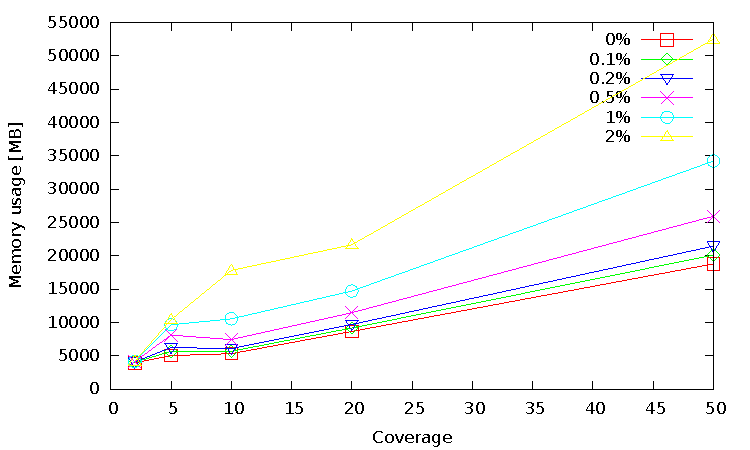
\includegraphics[width=16.5cm]{staphyl}
    \caption{Závislosť spotreby pamäte na pokrytí pre rôznu chybovosť vstupnej sady readov.}
    \label{fig:graf_staphyl}
\end{figure}

\subsection{Test na reálnych dátach}
% graf realne data, variujem coverage (samplovanim nasimulujem ine converages)

\section{Zhrnutie a interpretácia výsledkov}

\todo{nekonzistentnost oznaceni, superstring je raz ss a raz S}\\
\todo{zmenit \emph{ready} na ready} \\
\todo{usamova minimovka - citacie} \\
\todo{usamova minimovka - 1.1 shortest common superstring je np-hard + 2.5 apx.(?)} \\
\todo{mensie odstavce} \\
\todo{vyhodit slovo 'nejak'}
        
    \chapter*{Záver}
        \markboth{\MakeUppercase{Záver}}{}
        \addcontentsline{toc}{chapter}{Záver}
        \emph{Záver\ldots}

    \newpage
        \renewcommand{\refname}{Zoznam použitej literatúry}
        \markboth{\MakeUppercase{Literatúra}}{}
        \phantomsection
        \addcontentsline{toc}{chapter}{Zoznam použitej literatúry}
        \begin{thebibliography}{99}
 
    \bibitem[BB13]{BB13}
        Broňa Brejová,
        \emph{Skriptá k predmetu vyhľadávanie v texte},
        FMFI UK,
        2013.
        
    \bibitem[BV11]{BV11}
        Broňa Brejová a Tomáš Vinař,
        \emph{Metódy v bioinformatike},
        FMFI UK,
        2011.
        
    \bibitem[BW94]{BW94}
        Michael Burrows and David J Wheeler,
        \emph{A block-sorting lossless data compression algorithm},     
        Technical Report 124,
        1994.
        
    \bibitem[FM00]{FM00}
        Paolo Ferragina and Giovanni Manzini,
        \emph{Opportunistic data structures with applications},
        Proceedings of the 41st Annual Symposium on Foundations of Computer
        Science, strany 390--398,
        2000.
        
    \bibitem[PTW01]{PTW01}
        Pavel A. Pevzner, Haixu Tang and Michael S. Waterman,
        \emph{An Eulerian path approach to DNA fragment assembly},
        Proc Natl Acad Sci USA
        2001.
        
    \bibitem[MM90]{MM90}
        Udi Manber and Gene Myers,
        \emph{Suffix arrays: a new method for on-line string searches},
        First Annual ACM-SIAM Symposium on Discrete Algorithms, strany 319--327,
        1990.
        
    \bibitem[AKO04]{AKO04}
        Mohamed Ibrahim Abouelhodaa, Stefan Kurtzb and Enno Ohlebuscha,
        \emph{Replacing suffix trees with enhanced suffix arrays},
        Journal of Discrete Algorithms 2,
        2004.
        
    \bibitem[NZC09]{NZC09}
        Ge Nong, Sen Zhang and Wai Hong Chan,
        \emph{Linear Suffix Array Construction by Almost Pure Induced-Sorting},
        2009 Data Compression Conference, strany 193--202,
        2009.
        
    \bibitem[KS03]{KS03}
        Juha Kärkkäinen and Peter Sanders,
        \emph{Simple Linear Work Suffix Array Construction},
        Automata, Languages and Programming. Lecture Notes in Computer Science
        2719, strana 943,
        2003.
        
    \bibitem[GGV03]{GGV03}
        Roberto Grossi, Ankur Gupta and Jeffrey Scott Vitter,
        \emph{High-order entropy-compressed text indexes},
        Proceedings of the 14th Annual SIAM/ACM Symposium on Discrete Algorithms, strany 841--850,
        2003.
        
    \bibitem[JS12]{JS12}
        Jochen Singer,
        \emph{A Wavelet Tree Based FM-Index for Biological Sequences in SeqAn},
        Master thesis,
        Freie Universit\"{a}t Berlin,
        2012.
        
    \bibitem[NP11]{NP11}
        Nicolas Phillipe, Mika\"{e}l Salson, Thierry Lecroq, Martine Léonard, Thér\`{e}se Commes and Eric Rivals,
        \emph{Querying large read collections in main memory: a versatile data structure},
        BMC Bioinformatics 2011, 12:242,
        2011.
        
    \bibitem[SD11]{SD11}
        Jared T. Simpson and Richard Durbin,
        \emph{Efficient de novo assembly of large genomes using compressed data structures},
        Genome Research 2012, 22: 549--556,
        2011.
        
    \bibitem[GBMP14]{GBMP14}
        Simon Gog, Timo Beller, Alistair Moffat and Matthias Petri,
        \emph{From Theory to Practice: Plug and Play with Succinct Data Structures},
        13th International Symposium on Experimental Algorithms, strany 326--337,
        2014.
        
    \bibitem[DFPB13]{DFPB13}
        Viraj Deshpande, Eric DK Fung, Son Pham and Vineet Bafna,
        \emph{Cerulean: A hybrid assembly using high
throughput short and long reads},
        13th Workshop on Algorithms in Bioinformatics,
        2013.
        
    \bibitem[ZS00]{ZS00}
        Z. Sweedyk
        \emph{A 2.5-approximation Algorithm for Shortest Superstring},
        SIAM Journal on Computing 29, strany 954--986,
        2000.

    \bibitem[GJ02]{GJ02}
        Michael Garey and David S. Johnson    
        \emph{Computers and intractability},
        W.H. Freeman,
        2002.
        
    \bibitem[GGV03]{GGV03}
        Roberto Grossi, Ankur Gupta and Jeffrey S. Vitter,
        \emph{High-Order Entropy-Compressed Text Indexes},
        14th Annual ACM-SIAM Symposium on Discrete Algorithms, strany 841--850,
        2003.        
    
\end{thebibliography}
    
\end{document}
